\section{Results}
\label{sec:c2_results}

With our 48 simulated mergers in hand, we try to determine scaling relations of global quantities such as the remnant and disk mass, highest temperature, etc., and look for homologies in the remnant profiles.  For our analysis, we use a cylindrical $(\varpi,\phi,z)$ coordinate system centered on the remnant core.  Properties on the equatorial $(\varpi,\phi)$ plane -- defined as the original orbital plane -- are averaged over $\phi$ using particles within $\frac{1}{2}\hz$ of the equatorial plane, where \hz\ is the remnant's rotational axis ($\varpi = 0$) central scaleheight (see Sec.~\ref{sssec:c2_structuraltrends}).  Properties along the rotational $(z)$ axis are averaged within a cylinder $\varpi<\frac{1}{2}\hz$.  We use $\frac{1}{10}\hz$ as the bin size along both the equatorial plane and rotational axis.  We determine properties mostly as a function of enclosed mass $M(r)$, which we define spherically\footnote{Arguably, enclosed mass is more properly defined within equipotential surfaces, but this makes comparison with other simulations harder.  For dissimilar-mass mergers, the difference is slight.}.  Thus, we show, e.g., equatorial plane temperature $T(\varpi)$ as a function of $M(r=\varpi)$, the mass enclosed within a sphere with radius $r=\varpi$.

\subsection{Representative Mergers}
\label{ssec:c2_samplingofmergers}

\begin{figure}
\centering
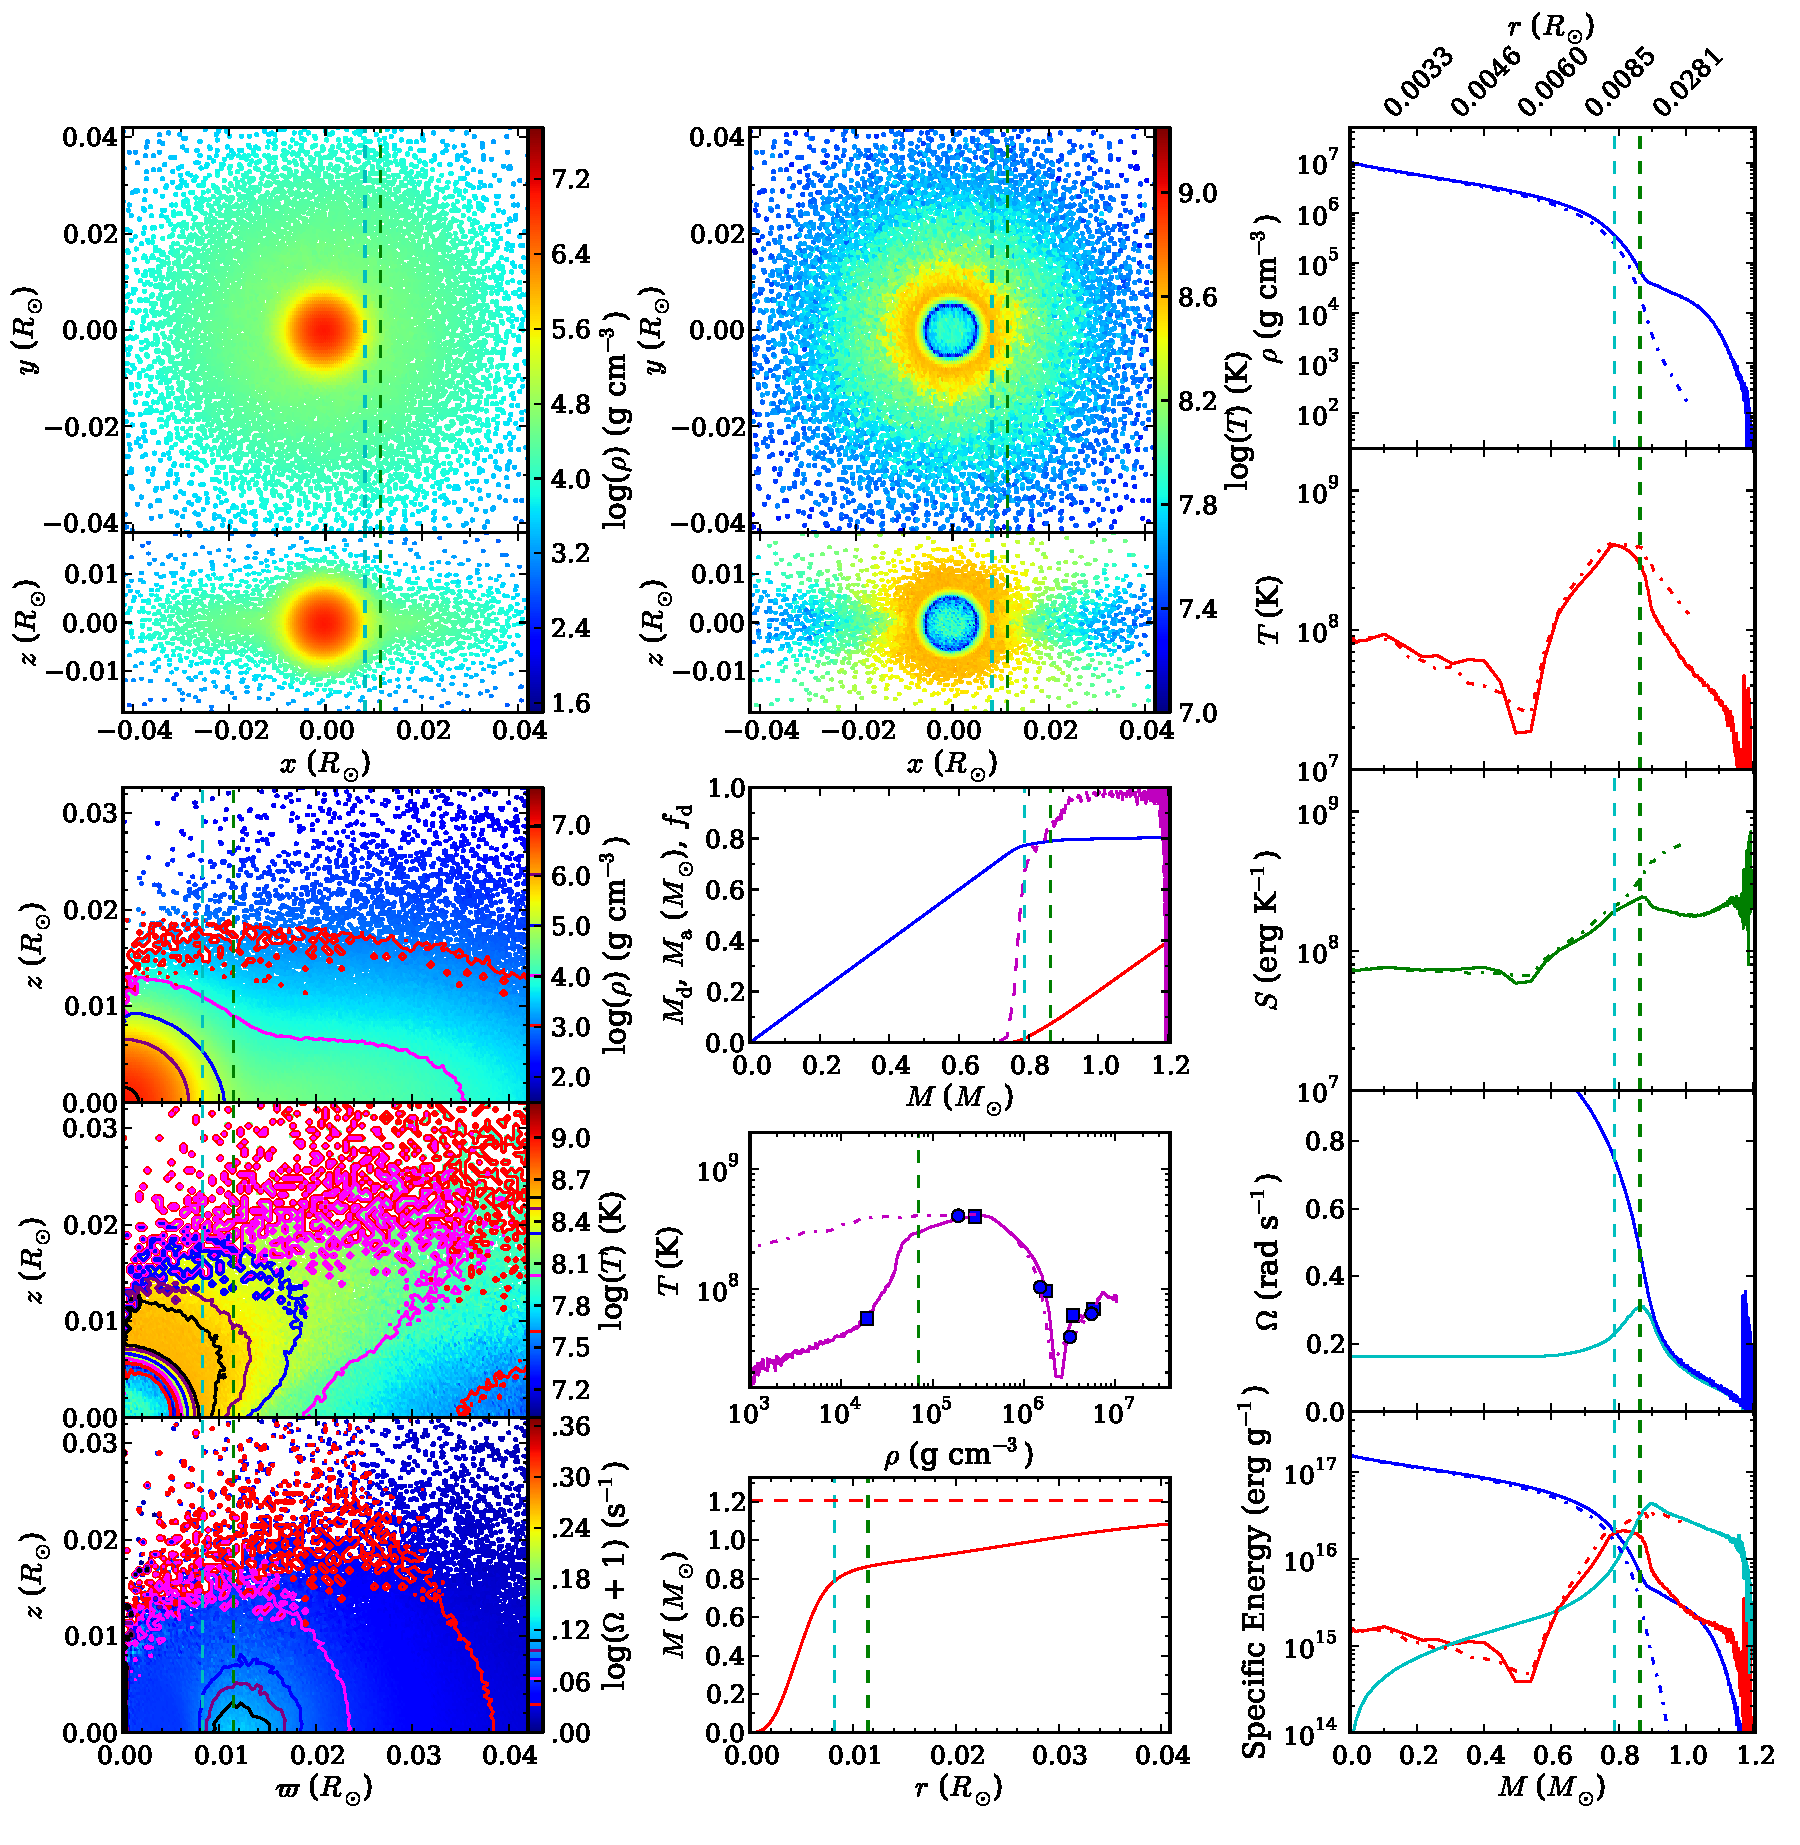
\includegraphics[width=1.0\columnwidth]{chapter2_zhu+13/figures/pt4pt8.pdf}
\caption{Structure of a 0.4 - 0.8 {\Msun} merger remnant, representing the general outcome of a merger of white dwarfs with dissimilar mass.  Upper left and middle -- binned maps of density $\rho$ and temperature $T$ along slices in the $xy$ and $xz$-planes.  Lower left -- binned maps and contours of density, temperature, and angular frequency $\Omega$ in the $(\varpi,z)$ plane, averaged over cylindrical coordinate $\phi$ and over $\pm z$ (with 1 added to $\Omega$ to avoid problems with the logarithmic intensity scale).  Middle -- enclosed masses of donor and accretor material {\Md} and {\Ma} (solid red and blue, resp.), and fraction of donor material \fdon\ at a particular mass shell (dashed magenta).  Middle, one but lowest -- temperature-density profile with enclosed masses in 0.2\,\Msun\ increments indicated, both along the equatorial plane (solid curve, squares) and along the rotational axis (dot-dashed curve, circles).  Middle, bottom -- enclosed mass as a function of $r$, with the total mass indicated by the horizontal dashed red line.  Right-hand column, top to bottom - density, temperature, entropy, angular (cyan) and Keplerian (blue) frequency, and degeneracy (blue), thermal (red) and rotational (cyan) specific energies as a function of enclosed mass $M$, both along the equatorial plane and along the rotational axis (solid and dot-dashed curves, respectively).  In all graphs, the start of the disk (where the centrifugal acceleration equals half the gravitational one) and the equatorial radius (or mass enclosed within) of maximum temperature are marked by vertical green and blue dashed lines, respectively. [{\em See the electronic edition of the Journal for Figs.~1.1--1.48}.]}
\label{fig:c2_mergersampling1}
\end{figure}

\begin{figure}
\centering
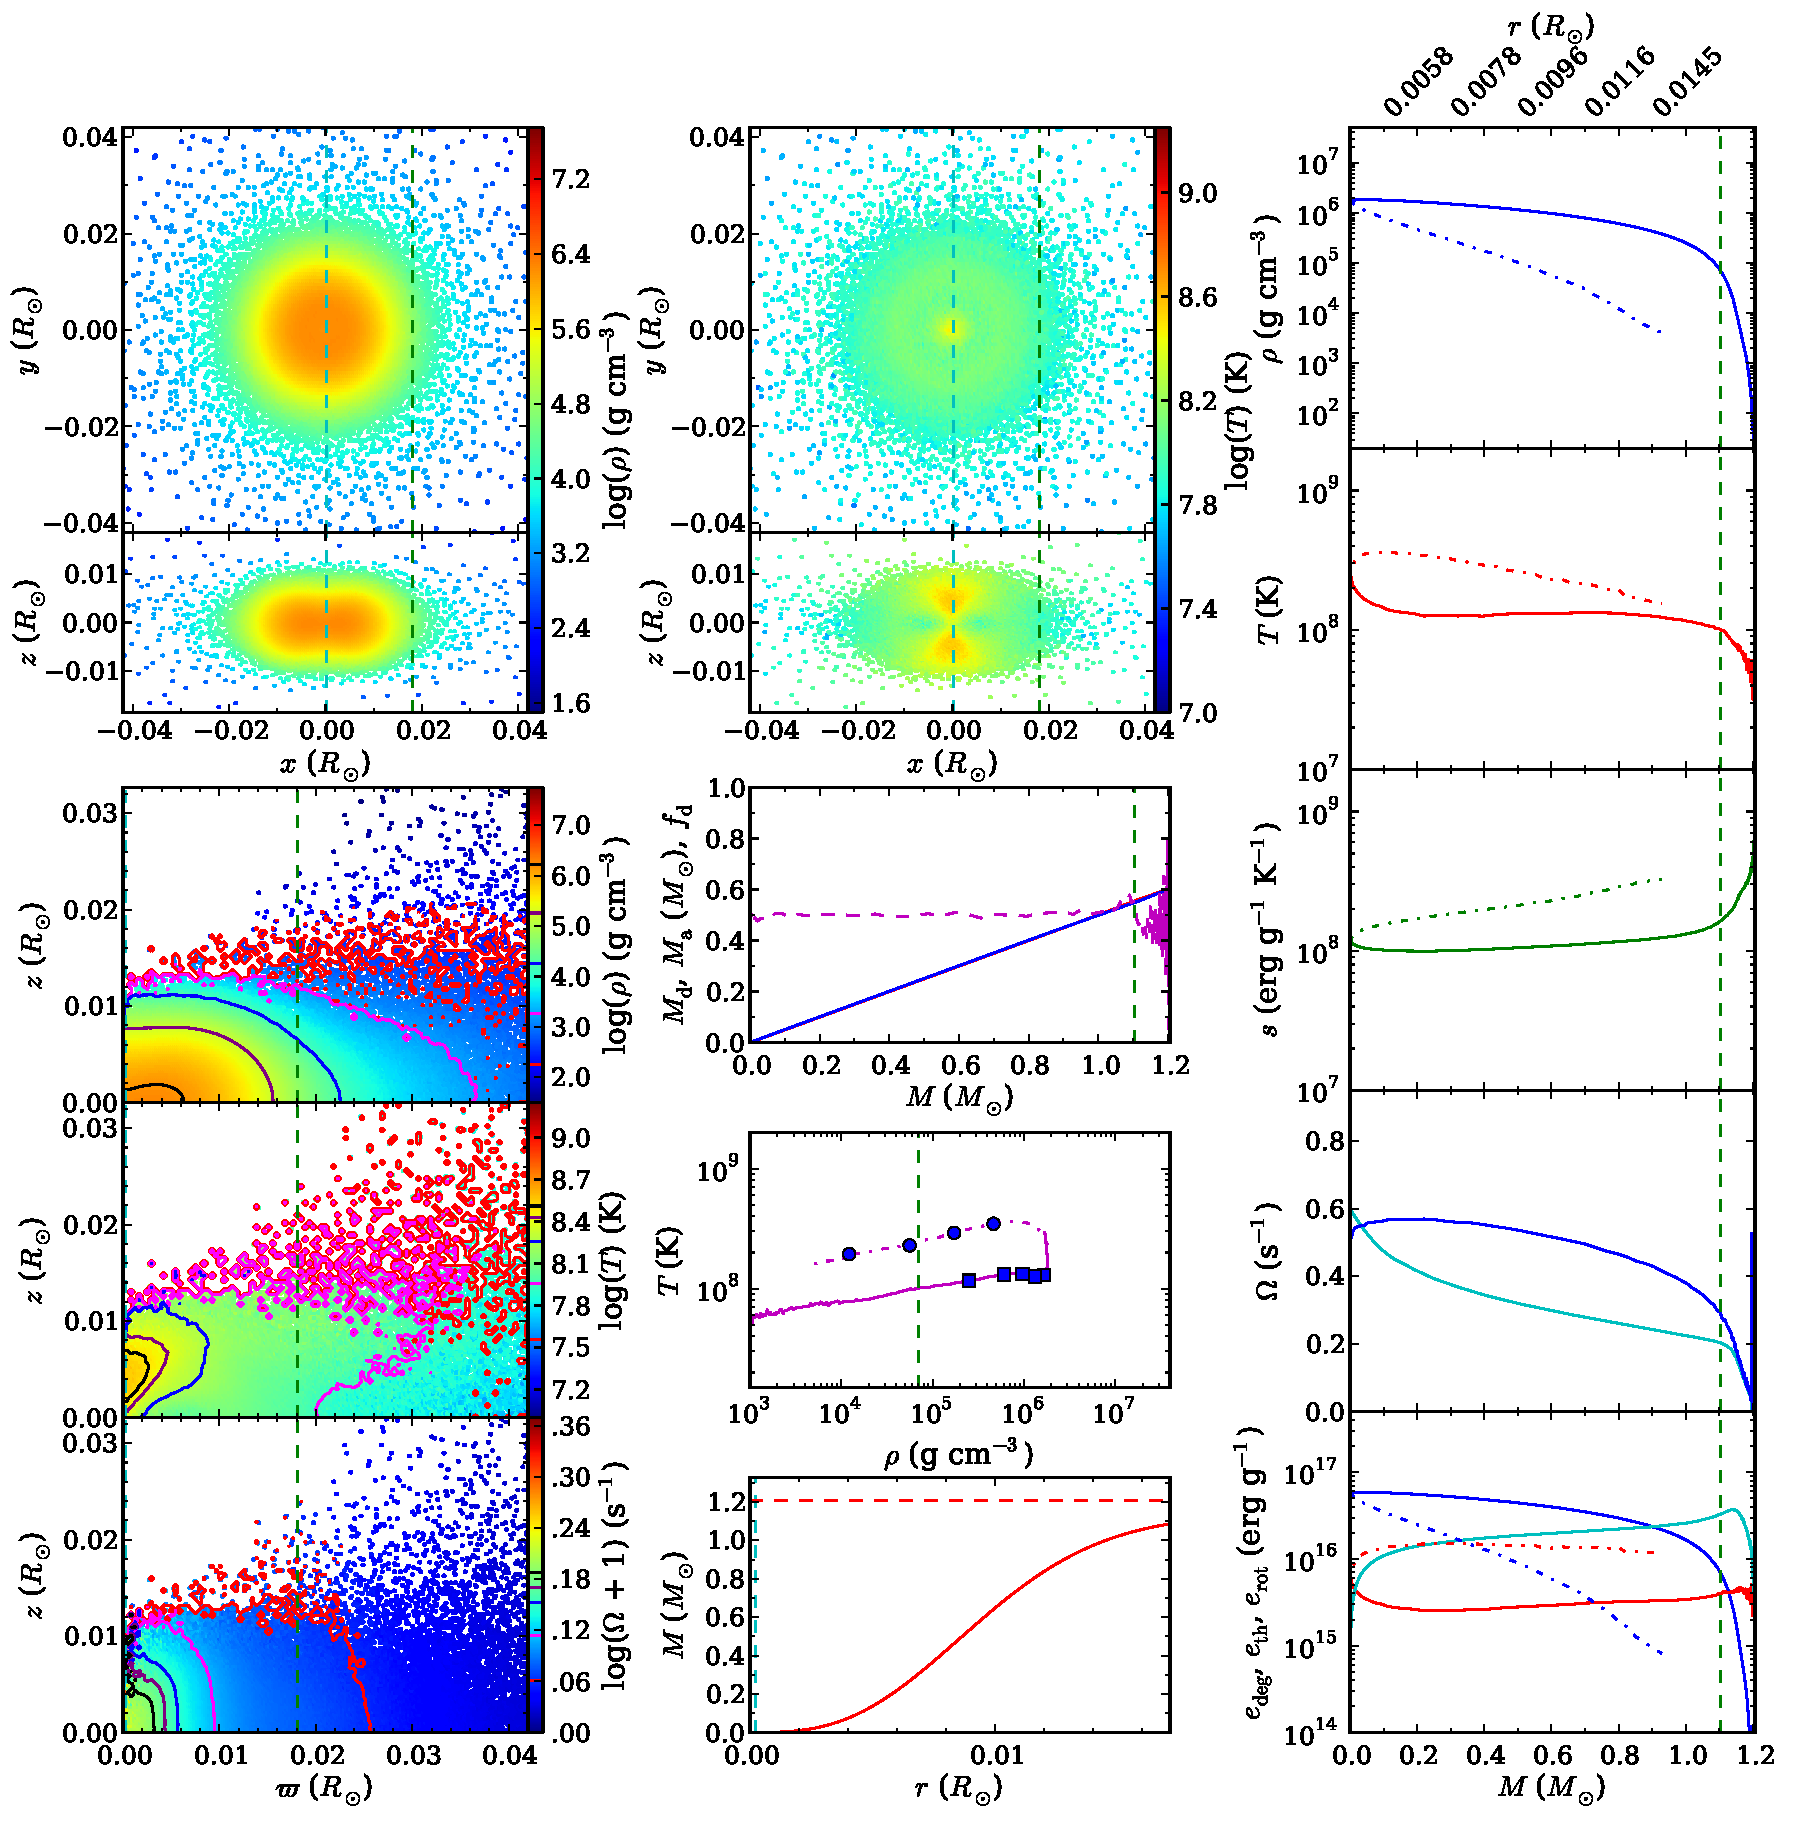
\includegraphics[width=1.0\columnwidth]{chapter2_zhu+13/figures/pt6pt6.pdf}
\caption{As Fig. Set~\ref{fig:c2_mergersampling1}, but for a 0.6 - 0.6 \Msun\ merger remnant, representing the general outcome of a similar-mass merger.}
\label{fig:c2_mergersampling2}
\end{figure}

As found for previous simulations, qualitatively the most important factor controlling the merger outcome is whether the WD masses are ``dissimilar'' or `` similar''.  In the former case, where the donor is significantly less massive than the accretor, only the donor overflows its Roche lobe,\footnote{The lower mass WD is larger and thus always fills its (smaller) Roche lobe first.} is disrupted, and accretes onto the accretor.  The accreted material is heated on impact, lifting degeneracy.  Hence, the merger remnant consists of a partly non-degenerate hot envelope and small, thick sub-Keplerian disk, both surrounding a cold core containing the largely unaffected accretor.

In the latter case of a similar-mass merger, there is a large degree of mixing between the two stars.  For exactly equal masses, both stars are disrupted simultaneously, and their accretion streams impact each other near the system's barycenter.  Material from the centers of both stars initially forms a thick, cold, dense torus orbiting the barycenter; this torus slowly shrinks due to viscous drag, pushing the accretion stream material above and below the equatorial plane.  When the stars have slightly different mass, the lower-mass one disrupts first, forming an accretion stream (or series of streams) that mixes with accretor material down to the center of the accretor (regardless of whether or not the other also disrupts).

We show the differences between similar and dissimilar-mass merger remnants using two representative examples in Figs.~\ref{fig:c2_mergersampling1} and~\ref{fig:c2_mergersampling2}: a 0.4 - 0.8 {\Msun} highly dissimilar and a 0.6 - 0.6 {\Msun} equal-mass merger, respectively.  One sees that the remnant morphologies are very different, consistent with previous work.  The 0.4 - 0.8 {\Msun} merger features a cold, nearly non-rotating and thus spherically symmetric remnant core, surrounded by a hot envelope with roughly equal degeneracy and thermal support, which itself is surrounded on the equatorial plane by a rotationally supported non-degenerate thick disk that holds most of the angular momentum.  The accretor forms the core, largely undisturbed by the merger, while the envelope and disk are composed almost entirely out of donor material.  The hottest points are on the interface between the core and the envelope.\footnote{The higher temperatures near the core are spurious; see Sec.~\ref{ssec:c2_spheat}}  The 0.6 - 0.6 {\Msun} remnant, on the other hand, has a massive, hot, partly rotationally supported and thus ellipsoidal core, and a very small but thick disk, both of which consist of material from both stars.  No distinct envelope is formed.  The hottest points are within the remnant core, just above and below the equatorial plane, arising from accretion stream material pushed out by the shrinking dense torus.

%MHvK: I think the mixing is already implicit in the above, and is better described as part of the discussion of nearly equal vs unequal below
%Mixing is another difference between these classes of mergers.  We show  the cumulative mass of the donor and accretor in the second column, third row plot in Figs. \ref{fig:c2_mergersampling1} and \ref{fig:c2_mergersampling2}.  For the unequal mass case, the cumulative mass curve of the donor only becomes non-zero when the cumulative mass of the accretor asymptotes, indicating negligible mixing, while for the 0.6 - 0.6 {\Msun} merger the two curves lie nearly on top of one another, indicating uniform mixing. 

%Comparison with other equal and unequal mass mergers show that the qualitative features of the 0.4 - 0.8 {\Msun} remnant extend to all unequal mass mergers, while those of the 0.6 - 0.6 {\Msun} remnant all equal mass mergers.

%MHvK: this belongs in caption
%Different colors represent different donor masses: red = 0.4 {\Msun}, orange = 0.5 {\Msun}, lime = 0.55 {\Msun}, green = 0.575 {\Msun}, cyan = 0.6 {\Msun}, sky blue = 0.625 {\Msun}, blue = 0.64 {\Msun}, dark blue = 0.65 {\Msun}, magenta = 0.7 {\Msun}, purple = 0.8 {\Msun}, brown = 0.9 {\Msun} and black = 1.0 {\Msun}. 

A good way to visualize how mergers transition between dissimilar and similar-mass is to look at changes in the remnant properties with varying donor mass.  In Fig. \ref{fig:c2_constacc}, we show curves for accretors of 0.65 (left) and 1.0\,\Msun (right).  One sees that remnants of highly dissimilar-mass mergers, with mass ratio $\qm\equiv M_\mrm{d}/M_\mrm{a} \lesssim0.5$, have properties resembling the 0.4 - 0.8 {\Msun} merger: their donor and accretor barely mixed, their temperature curves have off-center hot plateaus, and their angular velocity profiles feature an off-center bump.  The equal-mass, $\qm=1$ cases resemble the 0.6 - 0.6 {\Msun} remnant: they have flat temperature profiles and centrally peaked angular velocity profiles.  Intermediate cases have intermediate profiles, with the bumps in the temperature and angular velocity profiles widening with increasing {\qm}.  The 0.4 - 0.8 {\Msun} and 0.6 - 0.6 {\Msun} remnants therefore lie at the extremes of what merger remnants look like.

%and all merger remnants studied fall on the continuum between these two extremes.  {\bf move this last sentence later}Note that the 1.0 {\Msun} accretor runs show more spurious heating than the 0.65 {\Msun} accretor runs.

The similarity between some of the curves for the 0.65 and 1.0\,\Msun\ accretors in Fig. \ref{fig:c2_constacc} suggests a homology.  The similarity is closest for mergers with the same mass difference $\Delta M$, as can be seen in Fig. \ref{fig:c2_deltamcomp}.
%As the homology is not exact, we have defined this as a ``quasi-homology.'' 
For equal-mass mergers, all profiles are similar, simply scaled by a factor that depends on the total mass (except the 1.0 - 1.0 {\Msun} merger; see below).  As $\Delta M$ increases, the profiles are slightly less similar: with increasing total binary mass, the degree of mixing decreases, and the temperature and angular velocity maxima drift to slightly lower fractional enclosed mass.  Nevertheless, the profiles still resemble one another far more closely than they resemble curves with other $\Delta M$.  The same holds for profiles along the rotational axis.

It may seem surprising that the controlling parameter between these approximate homologies is the mass difference $\Delta M$ rather than the mass ratio {\qm}.  Empirically, however, the case is clear: e.g., the 0.4 - 0.5 (second column, yellow) and 0.8 - 1.0 {\Msun} (third column, black) mergers have the same {\qm}, but different $\Delta M$, and their structures clearly differ from one another.  The same is true for the 0.4 - 0.6 (third column, cyan) and 0.6 - 0.9 (fourth column, brown) {\Msun} mergers.  As we discuss below, the similarity of mergers of similar $\Delta M$ likely reflects the close relation between the ratio of central densities and mass difference.  

Before discussing the homologies and trends further, we should note the one dramatic exception.  The 1.0 - 1.0 {\Msun} simulation differs fundamentally from its fellow $\Delta M\,=\,0$ mergers.  During the evolution of this system, unlike for all other equal-mass mergers, one WD was fully disrupted before the other, and as a result material from one star (arbitrarily designated the ``donor'' before the start of simulation, hence the ``inverted'' mixing profile in Figs.~\ref{fig:c2_constacc} and~\ref{fig:c2_deltamcomp}) preferentially resides near the center of the remnant.  This system also often appears as an outlier in Sec.~\ref{ssec:c2_mergertrends} below.  The 0.9 - 0.9 {\Msun} merger also did not have equal mixing between the two stars, though the difference is much smaller.  \cite{rask+12} noticed the same effect in their simulations, and concluded it reflected the fact that more massive WDs are much more concentrated and therefore harder to disrupt.  This seems a likely explanation.

%Hindsight (after submission?), extra runs with 0.05 difference?

\begin{figure}
\centering
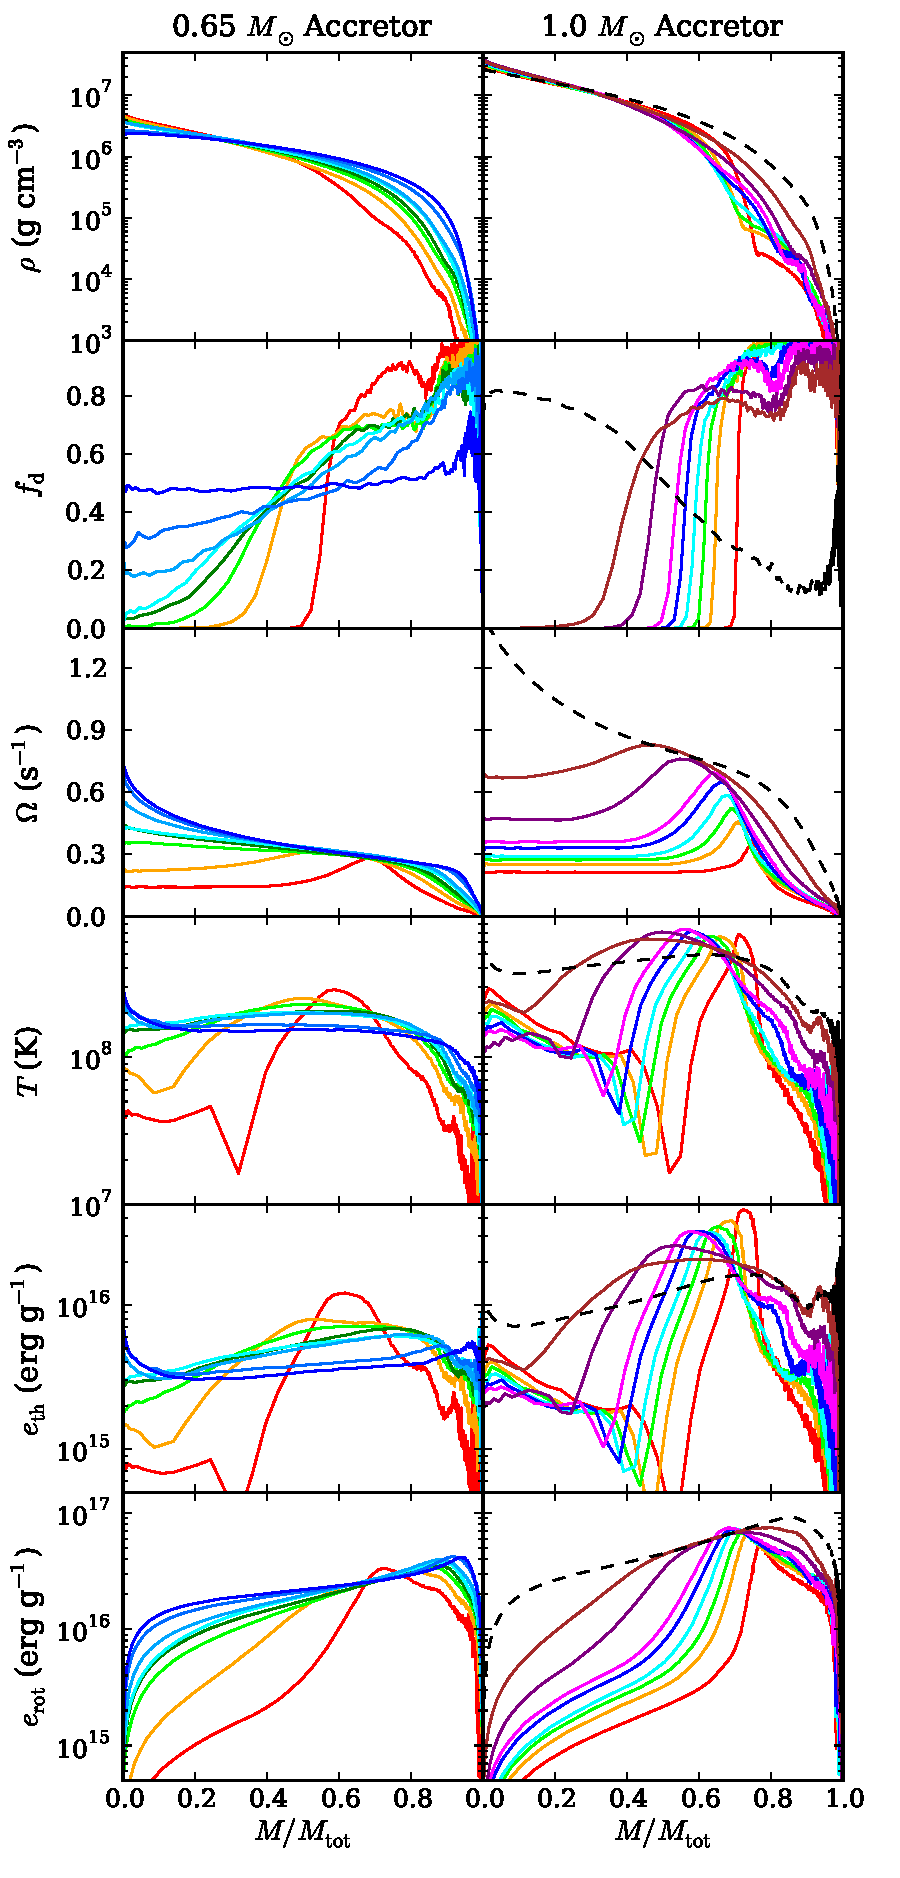
\includegraphics[angle=0,width=0.6\columnwidth]{chapter2_zhu+13/figures/constaccretorcomp.pdf}
\caption{Properties of mergers with 0.65\,\Msun\ (left) and 1.0\,\Msun\ (right) accretors, for donor masses of 0.4 (red), 0.5 (orange), 0.55 (lime), 0.575 (green), 0.6 (cyan), 0.625 (light blue), 0.64 (blue), 0.65 (dark blue), 0.7 (magenta), 0.8 (purple), 0.9 (brown), and 1.0\,\Msun\ (black).  Shown are, from top to bottom, density $\rho$, fraction of donor material \fdon, angular frequency $\Omega$, temperature $T$, specific thermal energy $E_{\rm th}$, and specific rotational energy $E_{\rm rot}$, all as a function of fractional enclosed mass $M/M_{\rm tot}$.  All properties are determined along the equatorial plane, except for \fdon\ which is defined spherically.  The 1.0 - 1.0 {\Msun} merger (dashed black line) is an outlier; see text.}
\label{fig:c2_constacc}
\end{figure}

\begin{figure}
\centering
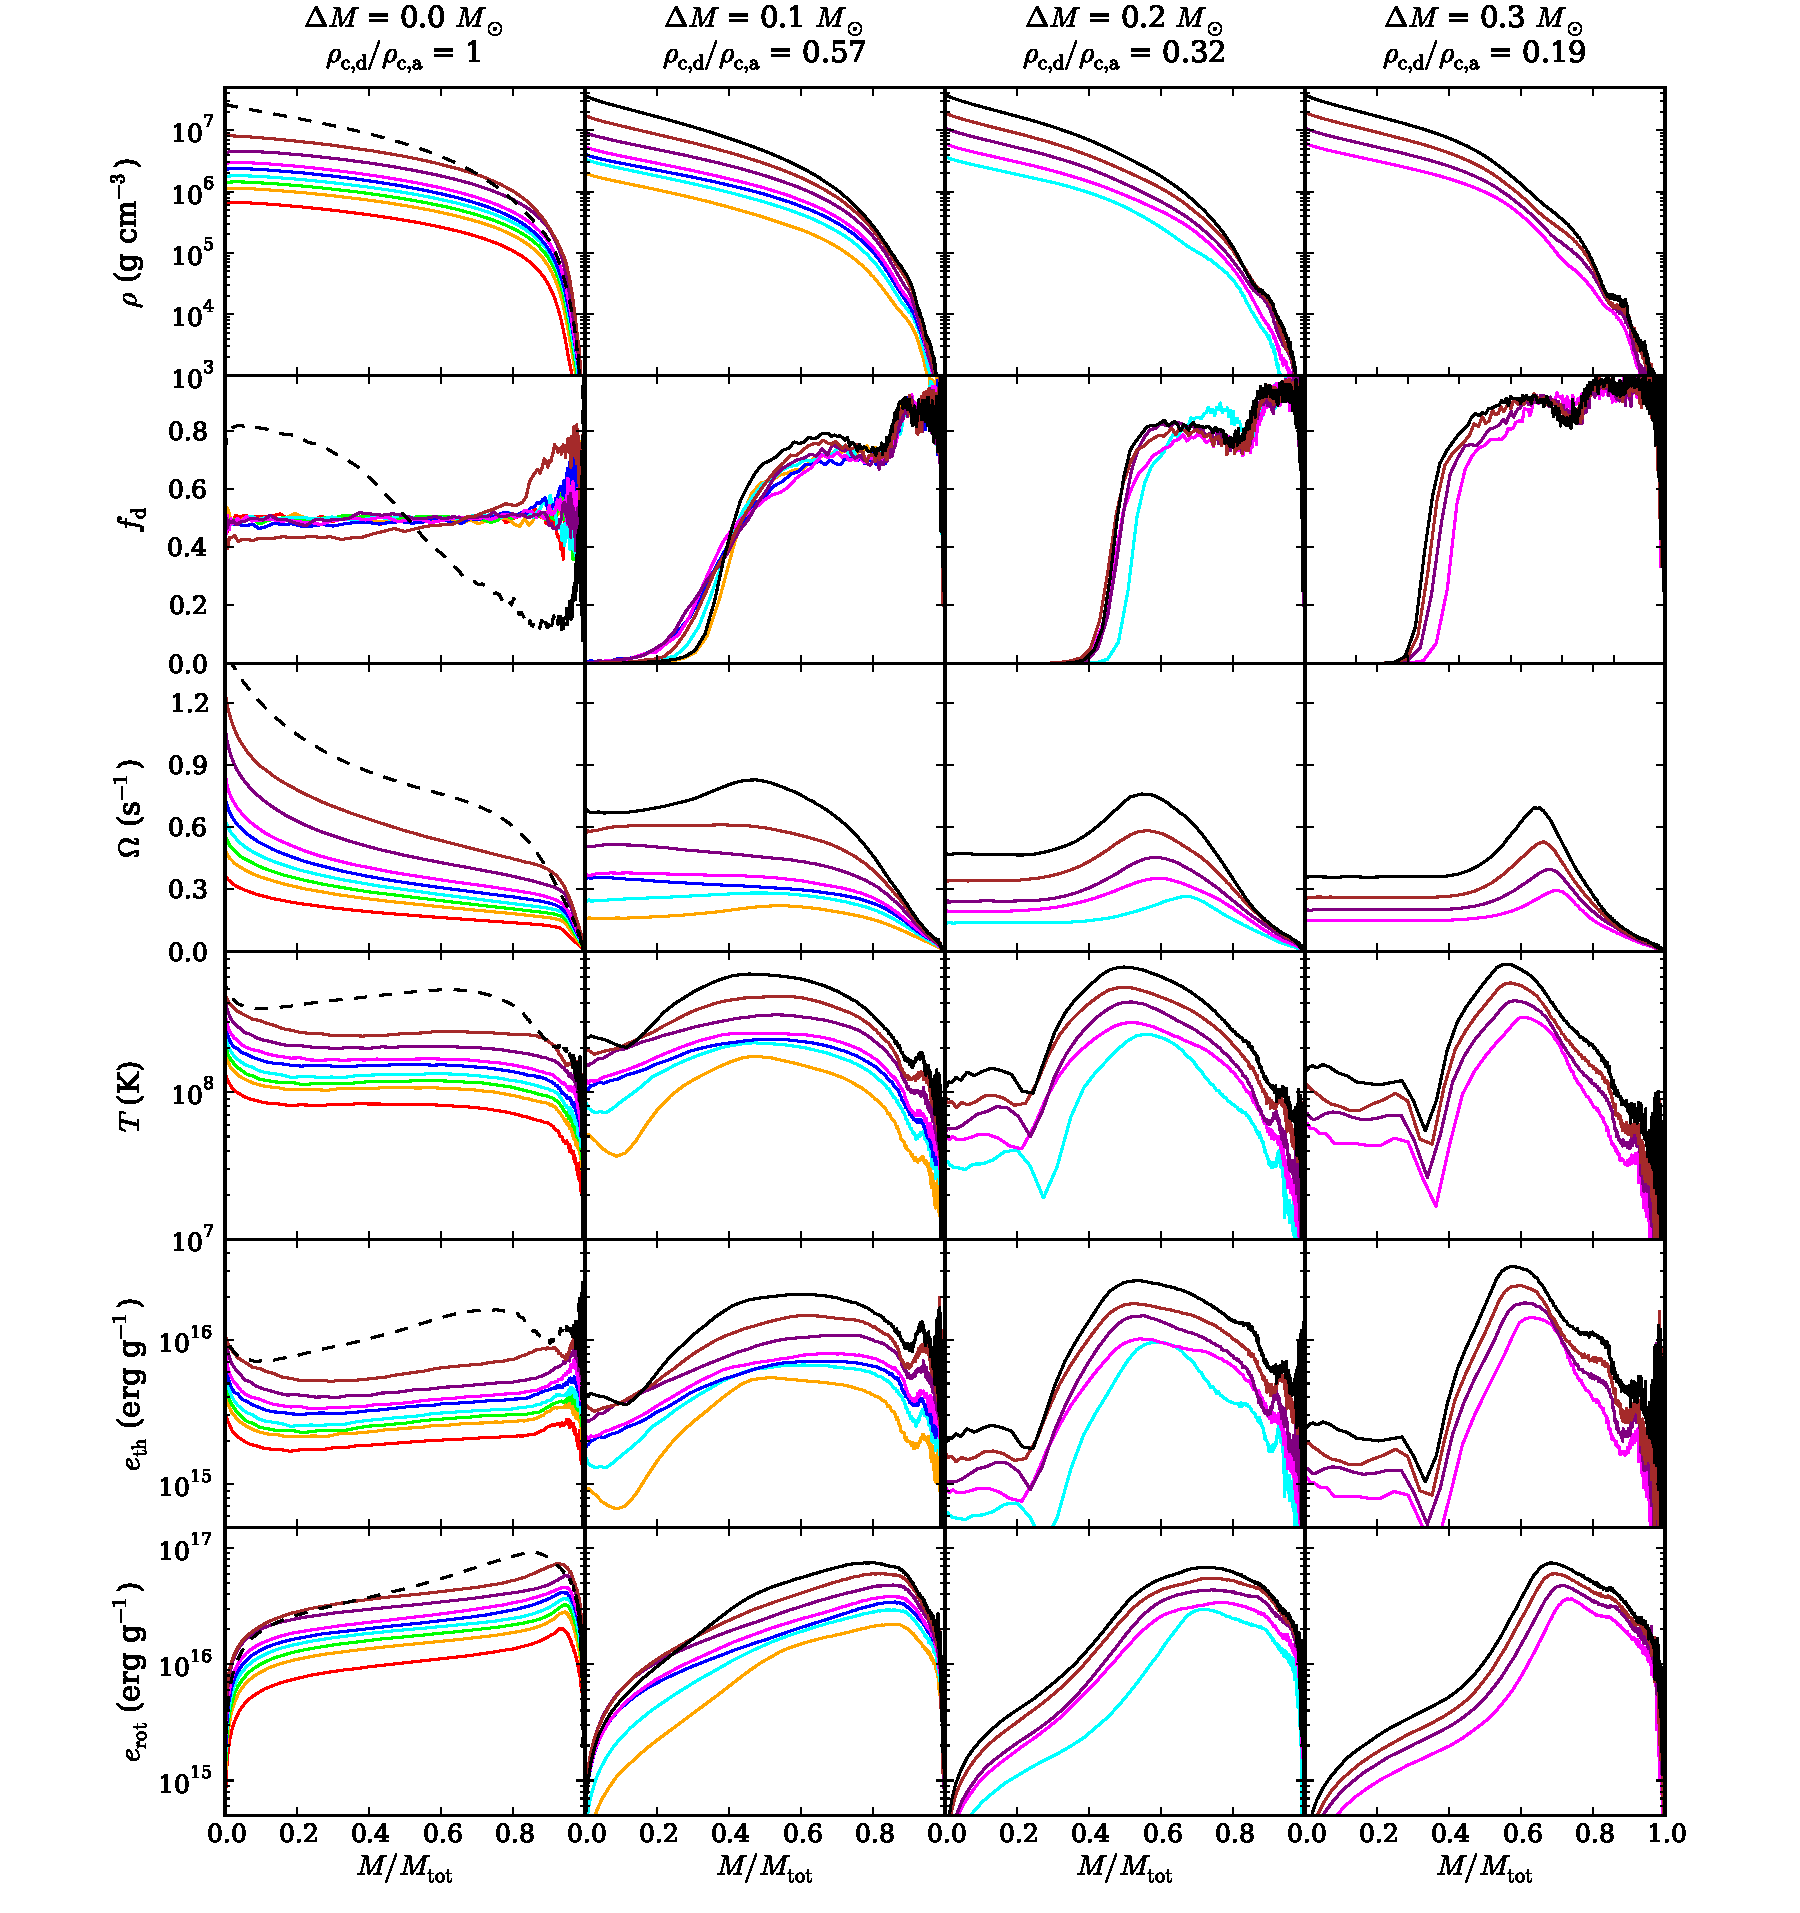
\includegraphics[angle=0,width=1.0\columnwidth]{chapter2_zhu+13/figures/deltamcomp.pdf}
\caption{Dependence of the properties of mergers on mass difference, with, from left to right, $\Delta M \equiv $ {\Ma} - {\Md} = 0.0, 0.1, 0.2, and $0.3\,\Msun$ mergers.  Properties shown, coloring, and line styles are as in Fig.~\ref{fig:c2_constacc}, except color represents accretor mass.}
\label{fig:c2_deltamcomp}
\end{figure}

\subsection{Merger Trends}
\label{ssec:c2_mergertrends}

A major goal of our work is to establish how various global properties of the merger remnant, such as remnant core and disk mass, maximum temperature, and maximum angular velocity, vary as a function of accretor and donor mass.  By quantifying these trends, we hope to help develop a parametrized model of merger remnants.  Before discussing trends, however, we stress that they are necessarily \textit{approximate} - second order effects, numerical noise and our choice of stopping time all affect the remnant properties.  Moreover, while integrated values like total thermal energy do not fluctuate from timestep to timestep, values at specific points in the remnant do (as noted the following sections).  For instance, the mass enclosed within the radius of peak equatorial temperature becomes ill-defined for similar-mass mergers because these have rather flat temperature profiles (Fig.~\ref{fig:c2_constacc}).  To partly mitigate these fluctuations, the values presented below were determined by averaging frames from the simulation over an eight second span, centered on the time corresponding to six orbits of the initial binary.

As might be expected from the approximate homologies described above, we found that many properties scaled well with $\Delta M$.  Of course, a scaling with a dimensional mass difference makes little sense; we believe its success reflects the fact that over the range of 0.4 -- 1.0\,{\Msun}, the central density {\rhoc} depends approximately exponentially on mass, with $\rho_{c} \simeq 3.3\times10^7{\rm\,g\,cm^{-3}} \exp[5.64(M/\Msun-1)]$ (see Fig.~\ref{fig:c2_mrho}).  Hence, a given mass difference $\Delta M$ corresponds to a given ratio of central densities, \rhocrat.  As argued in Sec.~\ref{sssec:c2_masstrends}, \rhocrat\ has a straightforward interpretation: it characterizes the degree of mixing between the donor and accretor.  We therefore discuss trends as a function of $\qrho\equiv\rhocrat$ from hereon.  Where necessary, we refer to the mass ratio as \qm.

%MHvK: superfluous after the above.
%We chose to plot every trend presented below as a function of {\qrho}.  This was not only because doing so makes comparisons between different trends easier, but also because due to the quasi-homology {\qrho}, i.e., $\Delta M$, parametrizes the majority of the trends presented.

\begin{figure}
\centering
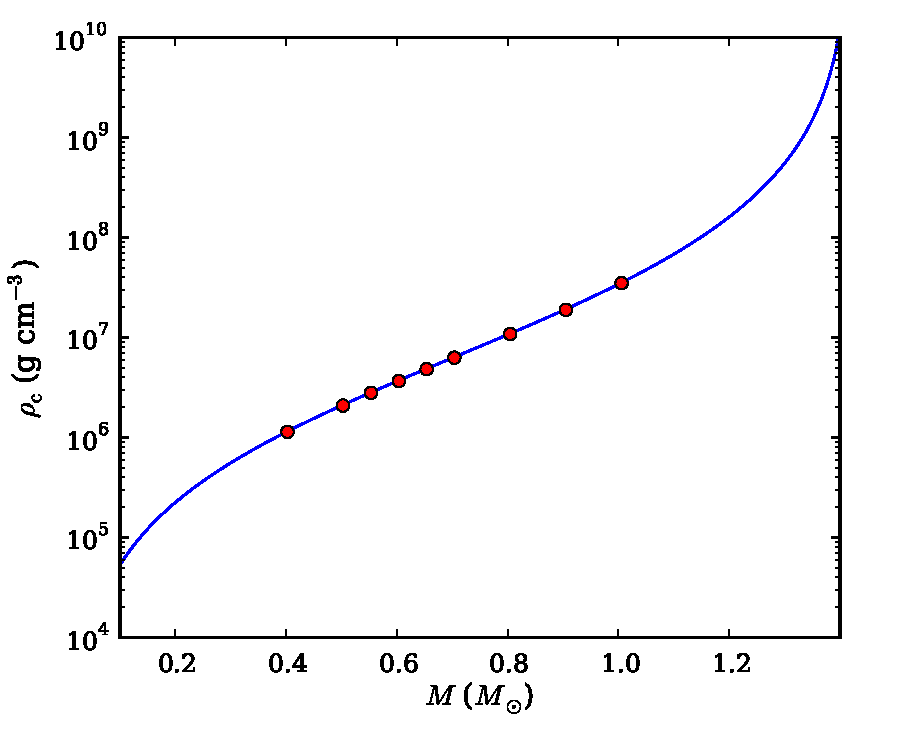
\includegraphics[angle=0,width=0.6\columnwidth]{chapter2_zhu+13/figures/Mrhorelation.pdf}
\caption{Relation between central density \rhoc\ and mass $M$ for carbon-oxygen white dwarfs, showing both the results of relaxing white dwarf models in Gasoline (red points), and integrating hydrostatic equilibrium directly for spherically symmetric, non-rotating CO WDs with $T=5\times 10^6\,$K (blue line).  For the mass range considered, the central density depends roughly exponentially on mass.}
\label{fig:c2_mrho}
\end{figure}

\subsubsection{What Constitutes Similar-Mass?}
\label{sssec:c2_whatisequalmass}

%\citeal{vkercj10}'s SN Ia channel is optimal when the hottest temperature in the merger remnant is at its center\qc{, i.e., equal-mass mergers}. 

As {\qrho} increases from a small value toward unity, the merger remnant's morphology shifts from resembling Fig.~\ref{fig:c2_mergersampling1} (dissimilar-mass) to resembling Fig.~\ref{fig:c2_mergersampling2} (equal-mass).  From Fig.~\ref{fig:c2_constacc}, ones sees that there is no particular {\qrho} at which one transitions from ``dissimilar'' to ``similar.''  Nevertheless, we can determine a rough critical value of~{\qrho} that separates mergers in which the core is largely unaffected from those in which it is changed significantly, a separation that likely affects the outcome of post-merger evolution.

%{\bf MHvK: note that I introduced new nomenclature, in the ratio of donor to accretor material.}
To determine the critical value, we show in Fig.~\ref{fig:c2_eqmass} the ratio of central to maximum temperature, $T_\mrm{c}/T_{\rm max}$, central to maximum angular velocity, $\Omega_\mrm{c}/\Omega_{\rm max}$, and the fraction of donor to accretor material within the central core, \fratio, where we define the central core as a sphere with radius \hz.  All three properties are measures of the extent to which the core has been affected: mixed regions tend to be hotter and more spun up, and contain material from both stars.

From Fig.~\ref{fig:c2_eqmass}, one sees that $\Omega_\mrm{c}/\Omega_\mathrm{max}$ approaches unity at $q_\rho\simeq0.6$; at higher values, the angular velocity profile has a plateau or central peak rather than an off-center bump.  Also at $q_\rho\simeq0.6$, \fratio\ starts to deviate from zero, i.e., donor material begins to penetrate the central core.  The temperature points show the transition is not abrupt: $T_\mathrm{c}/T_\mathrm{max}$ starts to deviate from its downward trend (which reflects spurious heating in the most dissimilar-mass mergers; Sec.~\ref{ssec:c2_spheat}) around $q_\rho\simeq0.3$ and continues to increase until $q_\rho=1.0$; at $q_\rho\simeq0.6$, $T_\mathrm{c}/T_\mathrm{max}\simeq0.5$.  Overall, this suggests that while the dependence is gradual, the morphology changes most around $\qrho\simeq0.6$.  This conclusion is confirmed by looking at the two-dimensional remnant temperature structures (Figs.~\ref{fig:c2_mergersampling1} and~\ref{fig:c2_mergersampling2}).  At $q_\rho\ll0.6$, the remnant core has a large, spherically symmetric cold region, the nearly unperturbed accretor.  This cold region shrinks with increasing \qrho, and at $q_\rho\simeq0.6$, spherical symmetry is broken.  For still larger \qrho, the cold region becomes a flat slice sandwiched between hotspots off the equatorial plane.

Given the above, we define ``similar-mass'' mergers as those with donor to accretor central density ratio $q_\rho>0.6$, and ``dissimilar-mass'' mergers as those with $q_\rho<0.6$.  This critical density ratio corresponds to a mass difference $\Delta M\simeq0.1\,\Msun$.

\begin{figure}
\centering
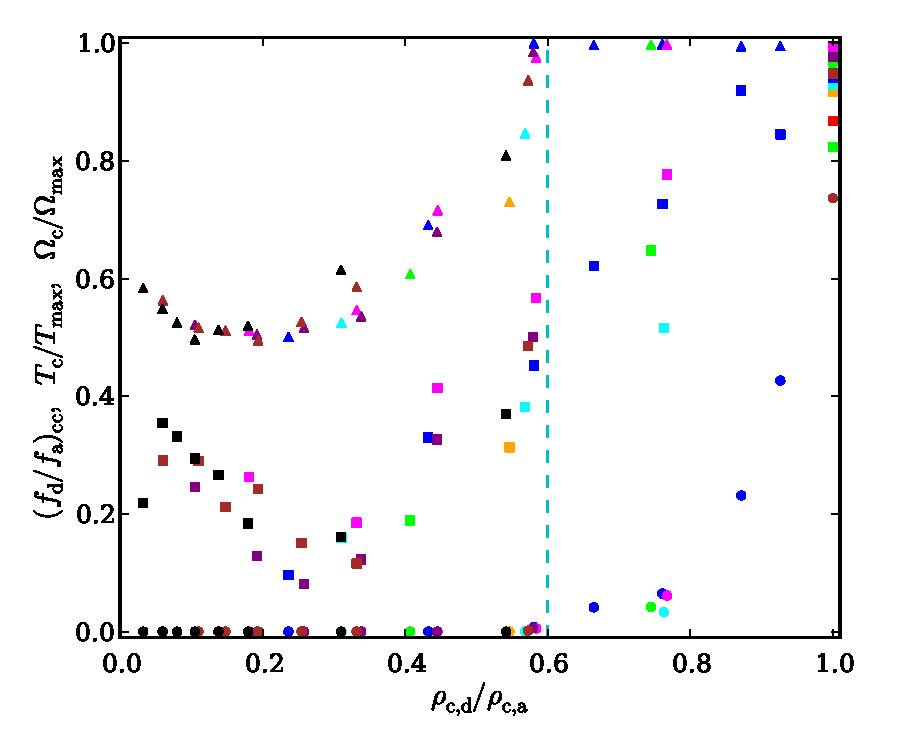
\includegraphics[width=0.6\columnwidth]{chapter2_zhu+13/figures/Eqmass.pdf}
\caption{Dependence of merger core properties on the ratio of the donor and accretor central densities, \rhocrat.  Shown are the ratio of central to maximum temperature $T_\mathrm{c}/T_\mathrm{max}$ (squares), central to maximum angular velocity $\Omega_\mathrm{c}/\Omega_\mathrm{max}$ (triangles), and central core donor to accretor mass fraction \fratio\ (circles), with colors representing different accretor masses, encoded as in Fig.~\ref{fig:c2_constacc}.  The vertical line marks $\qrho\equiv\rhocrat=0.6$, where $\Omega_\mathrm{c}/\Omega_\mathrm{max}$ reaches unity, \fratio\ becomes non-zero, and $T_\mathrm{c}/T_\mathrm{max}\simeq0.5$.  We suggest it separates ``dissimilar'' from ''similar'' mass mergers.}
\label{fig:c2_eqmass}
\end{figure}

\subsubsection{Structural Trends}
\label{sssec:c2_structuraltrends}

Here and in the following subsections of \ref{ssec:c2_mergertrends}, we describe various trends of remnant properties in detail, hoping to help attempts to interpolate between different simulations and motivate analytical and semi-analytical depictions of the merger.  Readers not requiring this level of detail may wish to skip to Sec. \ref{ssec:c2_qualitative}.  We begin our discussion of trends with size and density parameters.

\paragraph{The rotational axis central scaleheight.} We define the rotational axis central scaleheight \hz\ as the characteristic width $\sigma$ of a Gaussian fit to the density distribution along the $z$ axis at $\varpi = 0$.  \hz\ is a measure of the vertical extent of the remnant.  We find that the ratio $\hz/h_{\rm a}$, where $h_\mathrm{a}$ is the central scaleheight of the accretor, is reasonably well-approximated by,
\eqbegin
\frac{h_\mrm{z}}{h_\mathrm{a}} = 1.03 - 0.17\qrho^{1/2}
\qquad(\pm0.02),
\eqend
where the uncertainty listed in parentheses represents the root-mean-square (RMS) of the residuals around the approximation (see Fig.~\ref{fig:c2_structuretrends}a).  For highly dissimilar-mass mergers, \hz\ approximately equals the scaleheight of the accretor, while for similar-mass mergers, \hz\ is lower due to rotational support.

The vertical scaleheight increases with increasing $\varpi$: the scaleheight at the location of maximum temperature, $h(T_{\rm max})$, ranges from \hz\ to 1.21\hz, and the scaleheight at maximum angular velocity $h(\Omega_{\rm max})$ ranges from \hz\ to 1.88\hz.  The prefactor for both heights increases with increasing accretor mass {\Ma} and decreasing \qrho. 

\paragraph{The equatorial plane central scaleheight.}  Similar to \hz\, we define \hxy\ -- the characteristic width of a Gaussian fit to the density distribution along the equatorial plane -- as a measure of the equatorial extent of the remnant.  The ratio $\hxy/h_{\rm a}$ can be parametrized by
\eqbegin
\frac{\hxy}{h_{\rm a}} = 0.96 + 0.89q_\rho^2
\qquad(\pm0.08),
\eqend
where we excluded the 1.0 - 1.0 {\Msun} merger remnant for our fit (see Fig.~\ref{fig:c2_structuretrends}a).  The dependence on increasing \qrho\ reflects the increased rotational support of the remnant core.

\paragraph{The central density of the remnant.}  The central density, \rhoc, is always within a factor two of the central density of the accretor, \rhoca.  In Fig.~\ref{fig:c2_structuretrends}b, one sees that for given accretor mass, \rhocrhoct\ increases with increasing \qrho\ for highly dissimilar-mass mergers due to increasing compression of the remnant core, but begins to decrease because of increasing rotational support around $\qrho\simeq0.3$.  We could not find a simple parametrization for these curves.  Note that for some systems, as we continue running our simulations \rhocrhoct\ continues to increase.  As discussed in Sec.~\ref{ssec:c2_mergercomplete}, this is probably because artificial viscosity forces the merger remnant to undergo accelerated viscous evolution.

%\textbf{Actually I did find a term that can linearize central density: $M_\mathrm{a,enc}(\rho_\mathrm{d,c})/(M_\mathrm{a} - M_\mathrm{d})$ (i.e. the mass of material in the accretor with a higher density than the central density of the donor, scaled by $\Delta M$.  I don't have a clue as to what it means, though.}

%\end{itemize}

\begin{figure}
\centering
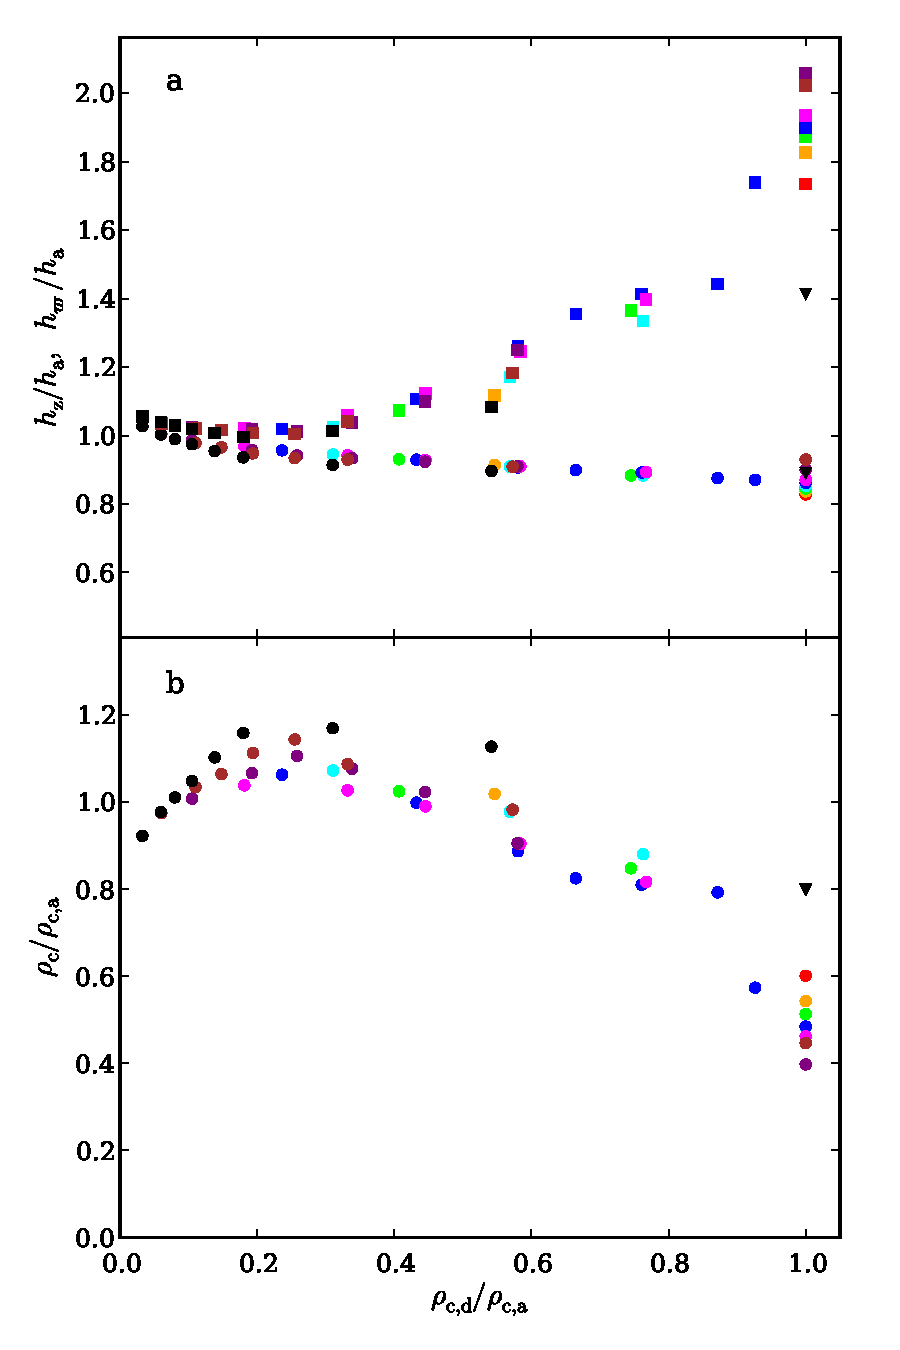
\includegraphics[angle=0,width=0.6\columnwidth]{chapter2_zhu+13/figures/StructureTrendsq.pdf}
\caption{Structural properties of mergers.  (a) Central scaleheights along the rotational axis (circles) and along the equatorial plane (squares) scaled to the scaleheight of the accretor, {\hz}/$h_\mathrm{a}$ and $\hxy$/$h_\mathrm{a}$.  (b) Central density of the merger remnant scaled to the central density of the accretor, {\rhocrhoct}.  Colors represent different accretor masses, encoded as in Fig.~\ref{fig:c2_constacc}.  Triangles represent the outlying 1.0 - 1.0\,\Msun\ merger.}
\label{fig:c2_structuretrends}
\end{figure}

\subsubsection{Mass Distributions}
\label{sssec:c2_masstrends}

The merger mixes material between the donor and accretor.  Here, we describe how this changes as a function of \qrho, as well as how the material is distributed between the pressure-supported core and envelope and the rotationally supported disk.

\paragraph{The masses of the core-envelope and disk.}  We formally define the core-envelope as the part of the remnant inside the inner disk radius $\varpi_\mrm{disk}$, i.e., that is supported primarily by pressure (degeneracy for the core, thermal for the envelope) and not rotation.  Since in every merger very little mass is ejected, a trend for either the core-envelope or the disk mass (\Mrem\ and \Mdisk, resp.) suffices to determine both.  The ratio of \Mrem\ to the accretor mass \Ma\ is well described by,
\eqbegin
\frac{\Mrem}{\Ma} = 1 + 0.81\qrho
\qquad(\pm0.03),
\eqend
if the 1.0 - 1.0 {\Msun} merger is neglected, and the fit's y-intercept is forced to unity.  See Fig.~\ref{fig:c2_restoftrends}a.

(see the dashed green line in Figs.~\ref{fig:c2_mergersampling1} and~\ref{fig:c2_mergersampling2})

\paragraph{The mass enclosing 50\% of the donor material.}  The further the donor penetrates, the smaller will be the mass enclosing half the donor's material, \MMfifty.  For mergers with $\qrho\lesssim0.8$, $\MMfifty/\Ma\,\simeq\,1.30$, with an RMS residual of 0.03 (Fig.~\ref{fig:c2_restoftrends}c).  We present this trend mostly because we discuss similar thermodynamic and rotational enclosed masses, but it is somewhat difficult to interpret physically, since \MMfifty\ increases with donor mass but decreases with mixing, which also depends on donor mass.  The trend is easier to interpret using enclosed accretor mass rather enclosed total mass, as done below.

\paragraph{The accretor mass enclosing 50\% of the donor material.}  As a different measure of the depth to which the donor penetrates, we consider just the accretor material within the mass enclosing half the donor, $\MMfifty-\frac{1}{2}\Md$.  This should equal the accretor mass if the donor is deposited above the accretor, and half the accretor mass if the two stars are completely mixed.  For $\qrho\lesssim0.8$, it can be approximated by (Fig.~\ref{fig:c2_restoftrends}b),
\eqbegin
\frac{\MMfifty-\frac{1}{2}\Md}{\Ma} = 1 - 0.190\qrho
\qquad(\pm0.009),
\eqend
where we forced the intercept to be unity.  In this regime, roughly half of the donor remains outside of the accretor, though the trend discussed next indicates that the other half which does penetrate the accretor is spread across a much larger region at higher \qrho.  When $q_\rho\gtrsim0.8$, the ratio drops sharply downward, indicative of the more thorough mixing expected for the similar-mass case.  However, the existence and exact location of this drop may be a function of initial conditions (see Sect.~\ref{ssec:c2_varyingazero}).  

\paragraph{The region over which the donor is spread.} As a measure of the thickness of the region affected by the merger, we use the difference of the mass enclosing 75\% of the donor material with that enclosing 25\% of the donor material, i.e., $\MMthick = M_{\rm enc}(\frac{3}{4}\Md) - M_{\rm enc}(\frac{1}{4}\Md)$.  Since 50\% of the donor is within this range, $\MMthick - \frac{1}{2}\Md$ is a measure of the amount of accretor mixed with the donor.  For $q_\rho\lesssim0.8$, the ratio of the latter to the total accretor mass follows,
\eqbegin
\frac{\MMthick-\frac{1}{2}\Md}{\Ma} = 0.30\qrho
\qquad(\pm0.02),
\eqend
while for $q_\rho\gtrsim0.8$ the trend curls upward until it reaches 0.5, the value expected for completely mixed remnants.  See Fig. \ref{fig:c2_restoftrends}d.

Combining the two above trends, we can formulate a qualitative picture of mixing.  For $q_\rho\lesssim0.8$, the donor can be thought of as being deposited onto the accretor and mixing with the accretor's outer layers, while for $q_\rho\gtrsim0.8$, the accretor also disrupts substantially, leading to a regime where both stars mix more uniformly.  The region over which the donor is spread, or thickness of the mixed layer, in both cases depends on {\qrho}, which suggests that the relative densities of the donor and accretor govern mixing, i.e., the donor mixes significantly with all accretor material up to some fraction of the central density of the donor.  Additional evidence of this will be seen in the thermodynamic trends below.  

One might consider an alternate picture in which the donor dredges up a constant fraction of its own mass in accretor material.  If this were the case, we would expect $(\MMthick-\frac{1}{2}\Md)/\Md$ to roughly be constant.  Our results, however, show that for $q_\rho\lesssim0.8$ this quantity is nearly a straight line that is close to zero for small \qrho\ ($(\MMthick-\frac{1}{2}\Md)/\Md = 0.35\qrho\pm0.02$).  This seems more consistent with mixing being determined by density.

%\begin{figure}
%\centering
%\includegraphics[angle=0,width=0.7\columnwidth]{MassTrendsq.pdf}
%\caption{Top: Mass enclosing half of the donor mass scaled to the accretor mass {\MMfifty}/{\Ma}.  Center: width of mixing scaled to the accretor mass ($\Delta M(M_\mathrm{d}) - \frac{1}{2}${\Md})/{\Ma}.  We define $\Delta M(M_\mathrm{d})$ as $M(0.75M_\mathrm{d}) - M(0.25M_\mathrm{d})$.  Right: remnant mass divided by accretor mass{\Mrem}/{\Ma}.  Colors (Fig. \ref{fig:c2_constacc} caption) represent different accretor masses.  Upside-down triangles represent points that are likely outliers.}
%\label{fig:c2_masstrends}
%\end{figure}

\begin{figure*}
\centering
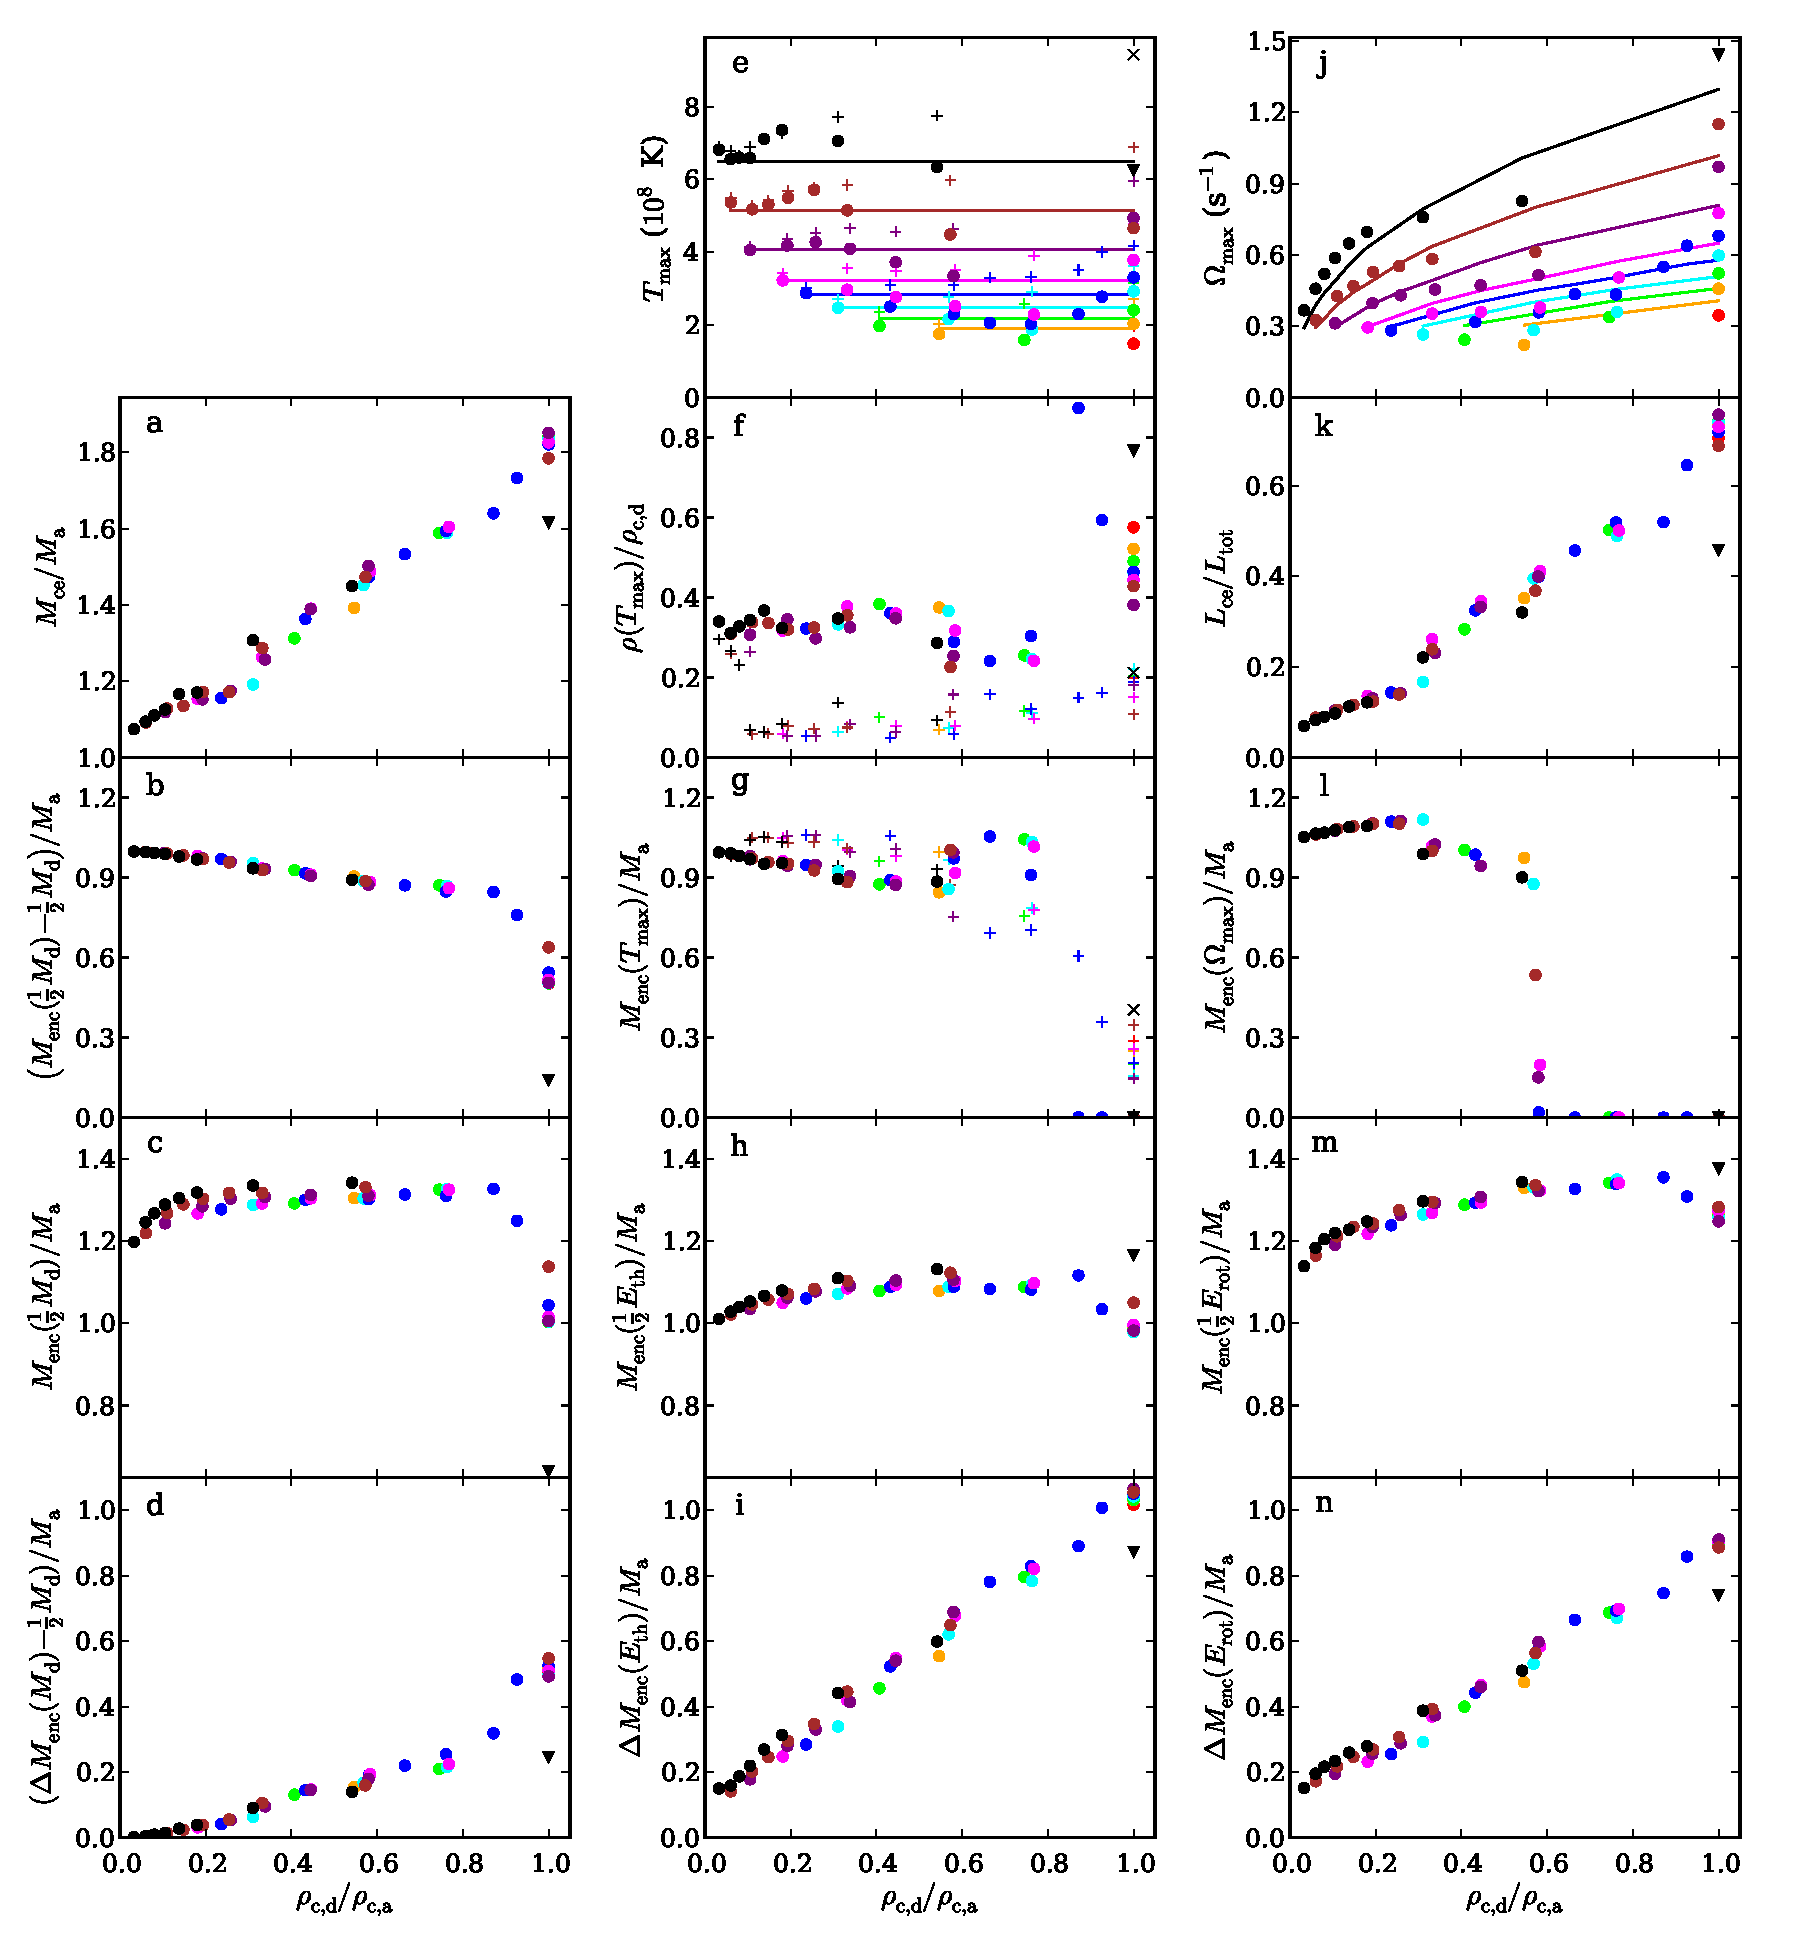
\includegraphics[angle=0,width=1.0\columnwidth]{chapter2_zhu+13/figures/RestofTrendsq.pdf}
\caption{Mixing, heating, and spin-up (left to right) for mergers. (a) Scaled mass of the remnant core-envelope (where scaling here and below is to the accretor mass).  (b) Fraction of the accretor within the mass enclosing half the donor mass.  (c) Scaled remnant mass enclosing half the donor mass.  (d) Fraction of the accretor mass within the region enclosing 25--75\% of the donor mass.  (e) Maximum equatorial temperature \Tmax\ (circles), with the approximation $\Tmax=0.20G\Ma m_\mathrm{p}/k_B\Ra$ overdrawn.  Maximum temperatures along the rotational axis are shown with crosses.  (f) Scaled density at the location of \Tmax\ (symbols as above).  (g) Scaled mass enclosed within the radius of \Tmax\ (symbols as above).  (h) Scaled mass enclosing half of the remnant thermal energy.  (i) Scaled mass of the region enclosing 25 -- 75\% of the remnant thermal energy.  (j) Maximum angular velocity \Omegamax\ (circles) with best fit $\Omegamax=3.8\Omega_\mrm{orb}$ overdrawn.  (k) Fraction of the angular momentum in the core-envelope.  (l) Scaled mass enclosed within the radius of maximum angular velocity.  (m) Scaled mass enclosing half of the total remnant rotational energy.  (n) Scaled mass of the region enclosing 25 -- 75\% of the remnant rotational energy.  Colors represent different accretor masses, encoded as in Fig.~\ref{fig:c2_constacc}.  Triangles represent equatorial plane values, and x-marks rotational axis values, of the 1.0 - 1.0\,\Msun\ merger.}
\label{fig:c2_restoftrends}
\end{figure*}

\subsubsection{Energy Balance}

The energy balance of the remnants indicate their primary means of support.  Since the remnants are virialized, we consider how the ratio of degeneracy, thermal, and rotational energy to the total internal energy of the remnants varies with \qrho.

\paragraph{Energy balance of the entire remnant.} The support against gravity changes from being due mostly to degeneracy pressure at low \qrho\ to having a substantial rotational contribution at $q_\rho\simeq1$.  This is because for highly dissimilar-mass mergers most of the internal energy is locked up within the accretor, which is hardly heated or spun up.  For similar-mass mergers, however, donor material mixes, to some degree, with the entire accretor, causing heating and spin-up throughout the entire remnant.

The total gravitational potential energy of the merger remnant can be described adequately by a constant fraction of $GM_\mrm{tot}^2/\Ra$,
\eqbegin
\frac{-E_\mathrm{pot}}{GM_\mrm{tot}^2/\Ra} = 0.49
\qquad(\pm0.01).
\eqend

%{\bf MHvK: I replaced the term internal energy with kinetic energy below, since it seems more appropriate; after all, molecular rotational or vibrational energy would be irrelevant.  CZ: in SPH ``kinetic'' seems to have an obvious definition, the speed of the particles, rather than the individual nuclei and electrons in the gas.  I feel the same is true for fluids in general, that the kinetic energy quantity naturally points to energy of bulk fluid flow.  I've left everything as is for now, but I feel it should be changed to internal.}

From the virial theorem, the internal energy should be related to the potential energy by $3(\langle\gamma\rangle - 1)E_\mathrm{I} = -E_\mathrm{pot}$, where $\langle\gamma\rangle$ is an appropriately averaged equivalent to the adiabatic index.  Since our remnants have cores where the electrons are becoming relativistic, one has $\langle\gamma\rangle$ somewhat smaller than $5/3$, especially for the more massive remnants.  We find that the ratio $E_\mathrm{I}/|E_\mathrm{pot}|$ can be described by,
\eqbegin
\frac{E_\mathrm{I}}{|E_\mathrm{pot}|} = 0.18\frac{M_\mathrm{a}}{M_\odot} + 0.42
\qquad(\pm0.01),
\eqend
which is $\sim$0.5 and $\sim$0.6 for low and high $M_\mathrm{a}$, respectively.  

The fraction of the internal energy carried by degeneracy and rotation is fairly well described by,
\begin{eqnarray}
\frac{E_\mathrm{rot}}{E_\mathrm{I}} &=& 0.31\qrho^{1/2}
\qquad(\pm0.01),\\
\frac{E_\mathrm{deg}}{E_\mathrm{I}} &=& 0.92 - 0.34\qrho^{1/2}
\qquad(\pm0.02).
\end{eqnarray}
With these, the fraction carried by thermal energy can also be calculated; as shown in Fig.~\ref{fig:c2_energytrends}a, the fraction in thermal energy first increases with increasing \qrho, but turns over at $\qrho\simeq0.7$, decreasing afterwards.  This reflects the competition between increased thermal energy from the two stars mixing, and increased rotational support from the spin-up of the core.  

Overall, for highly dissimilar-mass mergers, the internal energy is partitioned into degeneracy, rotational and thermal energy with a ratio of approximately 8:1:1, reflecting that, as stated above, such mergers are almost entirely supported by degeneracy pressure.  Similar-mass mergers, on the other hand, partition their internal energies with the ratio 6:3:1, i.e., rotational support is significant.  

\paragraph{Energy balance of the core-envelope.} Since the variations with \qrho\ seen for the remnant as a whole are almost entirely due to variations in the core and envelope rather than in the disk, the trends we find for the core-envelope are very similar to those we found above for the entire remnant,
\begin{eqnarray}
%\frac{-E_\mathrm{pot,ce}}{G\Ma\Md/\Ra} &=& 0.45
%\qquad(\pm0.02), \\
%\frac{E_\mathrm{I,ce}}{|E_\mathrm{pot,ce}|} &=& 0.182\frac{M_\mathrm{a}}{M_\odot} + 0.401
%\qquad(\pm0.009), \\
\frac{E^\mrm{ce}_\mathrm{rot}}{E^\mrm{ce}_\mathrm{I}} &=& 0.28\qrho
\qquad(\pm0.02), \\
\frac{E^\mrm{ce}_\mathrm{deg}}{E^\mrm{ce}_\mathrm{I}} &=& 0.94 - 0.32\qrho
\qquad(\pm0.02).
\end{eqnarray}
Note the dependency on \qrho, rather than on $\qrho^{1/2}$ as was found for the entire remnant.  See Fig.~\ref{fig:c2_energytrends}b.

\paragraph{Energy balance of the disk.} For the disk, we find very little dependence on \qrho, consistent with the idea that most of the changes in the partitioning of energy have to do with increased mixing between the donor and accretor, which affects the core and envelope much more than the disk.  Averaged over all mergers, we find
\begin{eqnarray}
\frac{E^\mrm{disk}_\mathrm{rot}}{E^\mrm{disk}_\mathrm{I}} &=& 0.74
\qquad(\pm0.03),\\
\frac{E^\mrm{disk}_\mathrm{th}}{E^\mrm{disk}_\mathrm{I}} &=& 0.19
\qquad(\pm0.02),\\
\frac{E^\mrm{disk}_\mathrm{deg}}{E^\mrm{disk}_\mathrm{I}} &=& 0.07
\qquad(\pm0.02).
\end{eqnarray}
Hence, the disk is composed of non-degenerate, primarily rotationally-supported material.  See Fig. \ref{fig:c2_energytrends}c.  (Note that we do not try to define a ratio of internal to potential energy of the disk or core-envelope, since the potential energy of either is not straightforward to determine.)

\begin{figure}
\centering
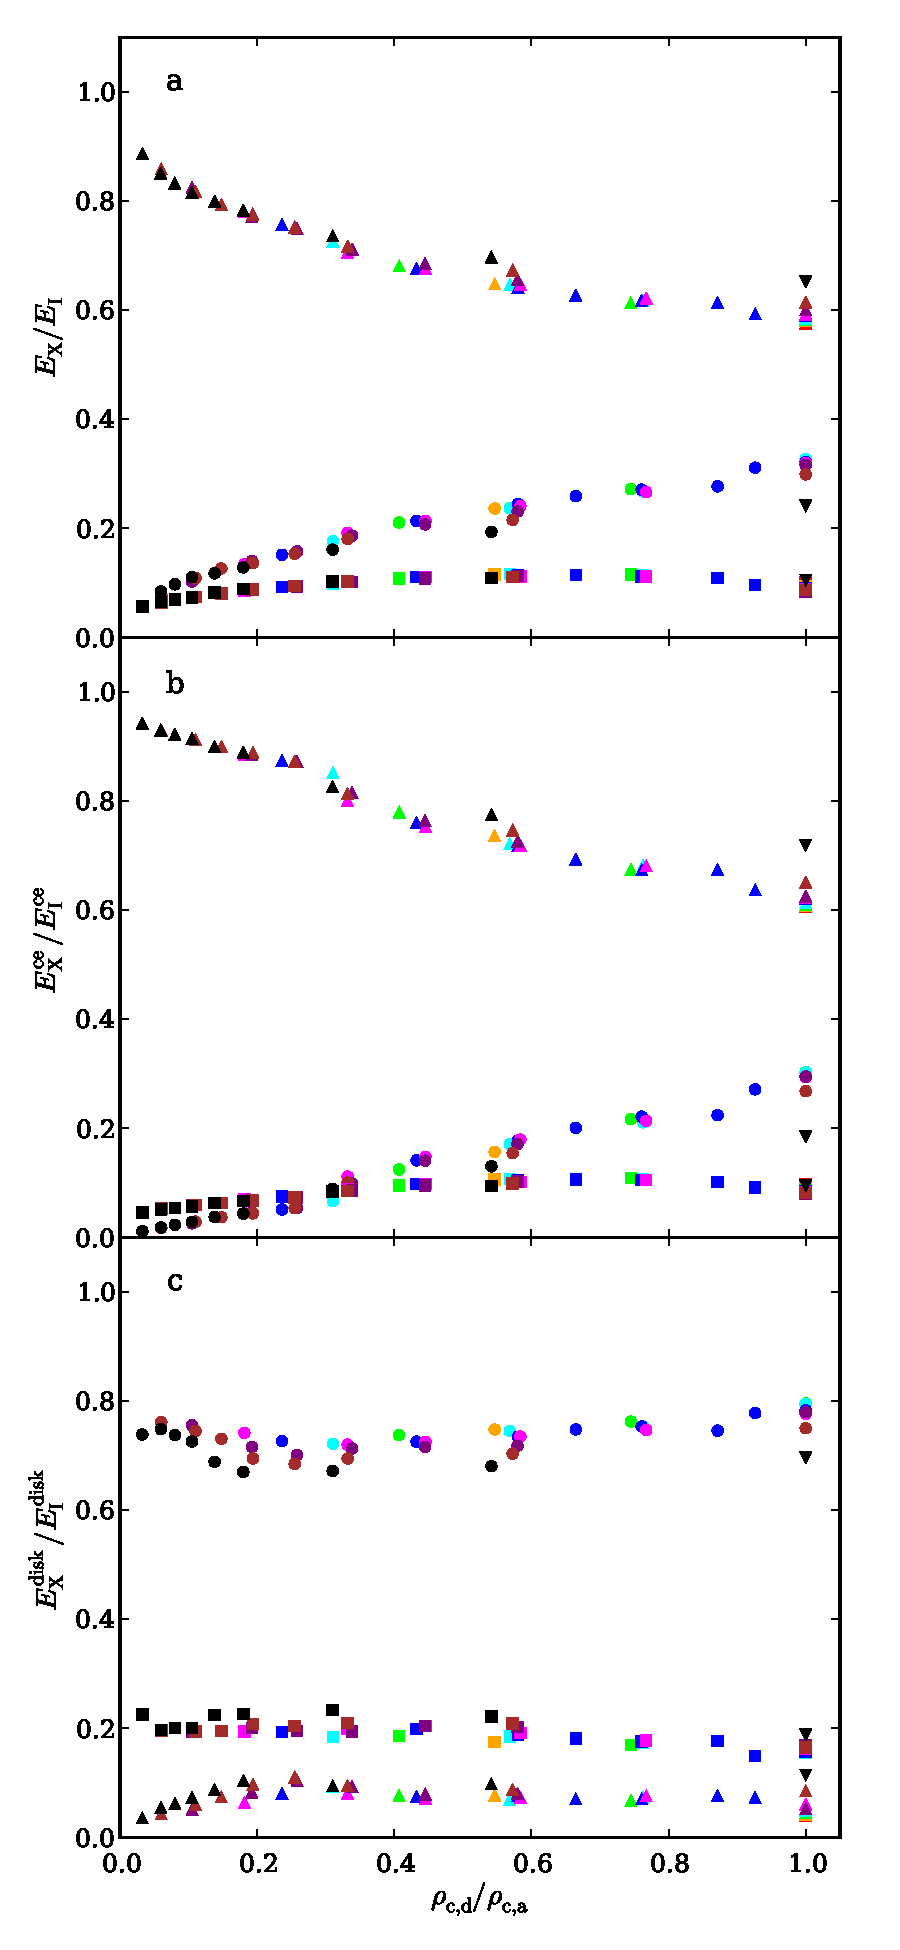
\includegraphics[width=0.6\columnwidth]{chapter2_zhu+13/figures/EnergyTrendsq.pdf}
\caption{Partition of energies in (a) the overall merger remnant, (b) the remnant core plus envelope, and (c) the remnant disk.  In each panel, the fraction of total energy carried in degeneracy (triangles), thermal (squares), and rotational (circles) energy is shown.  Colors represent different accretor masses, encoded as in Fig.~\ref{fig:c2_constacc}.  Triangles represent the 1.0 - 1.0\,\Msun\ merger.}
\label{fig:c2_energytrends}
\end{figure}

\subsubsection{Temperature and Thermal Energy}
\label{sssec:c2_thermtrends}

Since heating of the remnant is achieved through shocks and viscous dissipation, the most heavily mixed regions should also be the hottest.  We focus on equatorial thermodynamic values, but consider the rotational axis as well for similar-mass mergers.

\paragraph{The maximum temperature.} We find that the maximum temperature on the equatorial plane, \Tmax, scales with the potential of the accretor (Fig.~\ref{fig:c2_restoftrends}e),
\eqbegin
\frac{k\Tmax}{G\Ma m_\mathrm{p}/\Ra} = 0.20
\qquad(\pm0.03).
\eqend
This scaling is natural in the limit of highly dissimilar-mass merger -- for each nucleon, of order $G\Ma m_\mathrm{p}/\Ra$ is liberated and converted into thermal energy.  The temperature and thermal energy profiles in Fig.~\ref{fig:c2_constacc} show that with increasing {\qrho}, additional thermal energy is deposited into the remnant, but this energy is spread over a larger region, such that the maximum temperature remains roughly the same even as {\qrho} approaches unity.  

For a dissimilar-mass merger, the highest temperature along the rotational axis, \zTmax, is found at the tenuous outer edge of the hot envelope.  It is slightly higher than the maximum temperature found in the equatorial plane.  With increasing \qrho, however, the difference increases noticeably due to the two off-center hot spots found along the rotational axis in similar-mass mergers.  Fitting \zTmax, we find $k\zTmax/(G\Ma m_{\rm p}/\Ra) = 0.24\pm0.03$, though this does not capture the upturn for similar masses well.

All remnants with $q_\rho\gtrsim0.8$ have convectively unstable cores along the equatorial plane.  Artificially mixing these cores to make them isentropic decreases their maximum temperatures by 10 -- 50\% (not shown in Fig.~\ref{fig:c2_restoftrends}, but see the left panel of Fig.~\ref{fig:c2_willitexplode}).  All remnants are stable against convection along the rotational axis.

\paragraph{The density at the point of maximum temperature.}  For dissimilar-mass mergers, the density at the hottest equatorial point, \rhoTmax, depends mostly on the donor (see Fig.~\ref{fig:c2_restoftrends}f).  For $\qrho\lesssim0.5$, we find
\eqbegin
\frac{\rho(T_\mathrm{max})}{\rhocd} = 0.34
\qquad(\pm0.02).
\eqend
This proportionality again suggests that, at least for dissimilar-mass mergers, the donor mixes with the accretor up to a fraction of the central density of the donor, as alluded to earlier.  

At $\qrho\gtrsim0.6$, the dependence becomes less obvious, with \rhoTmax\ varying from $\sim\!25$ -- 90\% of \rhocd.  Since for these density ratios,  the donor material starts to penetrate the central core of the accretor -- and the accretor starts to disrupt as well -- the simple picture of the donor mixing up to a fraction of its own central density may be breaking down.  Furthermore, part of the spread in density reflects that for high \qrho\ the equatorial temperature profiles become nearly flat (see Fig.~\ref{fig:c2_constacc}, left column), thus increasing the sensitivity to noise in the determination of the location (but not the value) of maximum temperature.  This also affects our results for the enclosed mass, \MencTmax, below.

Since for dissimilar-mass mergers, \zTmax\ is located near the tenuous outermost regions of the hot envelope, where particle noise is high, the density at the point of maximum rotational axis temperature, \zrhoTmax\ (plus symbols in Fig. \ref{fig:c2_restoftrends}f), varies wildly between about \rhoTmax\ and one order of magnitude below \rhoTmax.  For similar-mass mergers, \zrhoTmax\ appears to be $\sim\!20$ -- 50\% of {\rhoTmax}.

\paragraph{The mass enclosed within the radius of maximum temperature.}  For dissimilar-mass mergers, the radius of maximum temperature occurs at an enclosed mass of $\MencTmax\simeq\Ma$, while for mergers with $\qrho\gtrsim0.8$, maximum temperature occurs at the center and $\MencTmax\simeq0$ (see Fig.~\ref{fig:c2_restoftrends}g).  For $\qrho\lesssim0.5$, we find
\eqbegin
\frac{\MencTmax}{\Ma} = 1-0.28\qrho
\qquad(\pm 0.01),
\eqend
where the fit's y-intercept is forced to unity.  Note that maximum temperature occurs near the bottom of the mixed zone, which is why \MencTmax\ is substantially smaller than \MMfifty.  The reasons it starts to deviate from a tight trend at $\qrho\simeq0.6$ are the same as those for \rhoTmax: the break-down of the simple mixing picture and the difficulty in determining the location of peak temperature for a broader plateau.

Since $\MencTmax<\Ma$, it may be surprising that \rhoTmax\ is not higher than \rhocd.  This is because the additional thermal and rotational support against gravity reduces the density gradient that would be required if degeneracy pressure were the only source of support.

For dissimilar-mass mergers, \zMencTmax\ is only slightly higher than \MencTmax, since the remnant core is nearly spherically symmetric, apart from the fact that the hot envelope is slightly more extended in the vertical direction.  For similar-mass mergers, the difference increases, reflecting the development of the off-center hot spots, until $\zMencTmax/\Ma\simeq0.25$ for equal-mass mergers.

\paragraph{The mass enclosing half the remnant thermal energy.}  As a more robust measure of where thermal energy is deposited during the merger, we consider the mass enclosing half the remnant thermal energy, \MEthermfifty\ (see Fig.~\ref{fig:c2_restoftrends}h).  We find this is very close to the mass of the accretor,
\eqbegin
\frac{\MEthermfifty}{\Ma}= 1.06
\qquad(\pm 0.04),
\eqend
if the 1.0 - 1.0 {\Msun} merger is neglected.  One sees turnovers at the extremes, for $\qrho\lesssim0.2$ and $\qrho\gtrsim0.8$.  The former likely is because thermal energy is deposited into a narrow strip right on the surface of the accretor, while the latter is probably due to the disruption of the accretor.

While smaller than \MMfifty, \MEthermfifty\ is always larger than \MencTmax.  This reflects that high density degenerate material has lower specific heat, so that for the same energy per unit mass the temperature is higher (see Fig.~\ref{fig:c2_constacc}).  

\paragraph{The width of the remnant thermal energy.}  The mass enclosed between the 25$^{\rm th}$ and 75$^{\rm th}$ percentiles of thermal energy, $\MEthermthick = M_{\rm enc}(\frac{3}{4}E_\mathrm{th}) - M_{\rm enc}(\frac{1}{4}E_\mathrm{th})$, is a measure of the extent of the remnant that has been heated (see Fig.~\ref{fig:c2_restoftrends}i).  Ignoring the 1.0 - 1.0 \Msun\ merger, it can be fit by,
\eqbegin
\frac{\MEthermthick}{\Ma} = 0.11+0.94\qrho
\qquad(\pm0.03).
\eqend
Here, we did not force the y-intercept to go to zero, which is expected physically but gives a substantially poorer trend.

%{\bf MHvK: please clarify the next sentence; what is the point?} {\MEthermthick} is also about \emph{DOUBLE???} the width of the ``bumps'' of high temperature seen in Fig.~\ref{fig:c2_constacc}.  

%\textbf{I don't think the 0.306 is physical.  For a zero-mass donor, {\MEthermthick} is non-zero (it doesn't matter how much thermal energy the accretor has, {\MEthermthick} will be non-zero), but describes something totally different than {\MEthermthick} during a merger.  Supposedly there's a transition zone between the zero-mass donor and our regime, where it describes the temperature bump, but since we have no data on this we can't say anything about this zone.  0.281, then isn't anything more than a way to make this section of the trend fit, and doesn't represent {\MEthermthick} for a zero-mass donor.}

%\begin{figure}
%\centering
%\includegraphics[angle=0,width=0.7\columnwidth]{ThermTrendsq.pdf}
%\caption{Top left: maximum equatorial temperature {\Tmax} with best fit {\Tmax} = $0.202GM_\mathrm{a}m_\mathrm{p}/(R_\mathrm{a}k_B)$.  Top right: equatorial density at the point where {\Tmax} occurs, {\rhoTmax}.  Middle left: mass enclosed within the radius containing {\Tmax}, {\MencTmax}.  Middle right: mass enclosing half of the remnant thermal energy scaled to the accretor mass, {\MEthermfifty}.  Bottom left: width of the remnant thermal energy $\Delta M(E_\mathrm{therm})$ normalized by the accretor mass.  Plus symbols represent values on the $z$-axis.  Colors (Fig. \ref{fig:c2_constacc} caption) represent different accretor masses.  Upside-down triangles and x symbols represent points on the $xy$-plane and $z$-axis, respectively, that are likely outliers; in particular the ``tails'' of the {\MEthermfifty} and $\Delta M(E_\mathrm{therm})$ plots are probably due to spurious heating.}
%\label{fig:c2_thermtrends}
%\end{figure}

\subsubsection{Angular Velocity and Rotational Energy}
\label{sssec:c2_rottrends}

For a dissimilar-mass merger, the donor carries most of the angular momentum.  As a result, the hot envelope contains more angular momentum and features higher angular velocities than the core, since the envelope is where most of the accreted donor material resides.  Spin-up of the accretor is accomplished through shocks, $PdV$ work and shearing forces.  For a similar-mass merger, the two stars carry similar amounts of angular momentum and thoroughly mix.  Conservation of angular momentum then implies that the entire remnant rotates rapidly.

\paragraph{The maximum angular velocity.}  On the equatorial plane, the highest angular velocity, \Omegamax, scales linearly with the orbital angular velocity of the pre-merger binary, $\Omegaorb = 2\pi/P_\mrm{orb}$ (see Fig.~\ref{fig:c2_restoftrends}j),
\eqbegin
\frac{\Omegamax}{\Omegaorb} = 3.8
\qquad(\pm0.6).
\eqend

\paragraph{The ratio of core-envelope to total angular momentum.} For more similar-mass mergers, more angular momentum is deposited in the accretor and ends up in the core and envelope (see Fig.~\ref{fig:c2_restoftrends}k).  The ratio of core-envelope to total angular momentum, \Lrat, is approximately,
\eqbegin
\frac{L_\mrm{ce}}{L_\mrm{tot}} = 0.70\qrho
\qquad(\pm 0.03),
\eqend
where we fit only for $\qrho > 0.25$ and ignore the 1.0 - 1.0 {\Msun} merger.  For $\qrho\lesssim0.25$, the trend becomes shallower, resulting in a non-zero intercept.  This suggests that even in cases where the donor has negligible mass some angular momentum is transferred to the accretor.

\paragraph{The mass enclosed inside the radius of maximum angular velocity.}  
%MHvK: don't like this trend at all!
%\eqbegin
%\M_\mathrm{enc}(\Omega_\mathrm{max}) = 1.25(M_\mrm{a} - \frac{1}{4}M_\mrm{d})\,%\,(\pm0.04)
%\eqend
%\noindent for $q_\rho < 0.55$.  
For dissimilar-mass mergers, both \MencOmax\ and \MencTmax\ are about equal to \Ma, with \MencOmax\ slightly larger than \MencTmax: for $\qrho\lesssim0.55$, $\MencOmax/\Ma\,=\,1.05\pm0.06$.  This is consistent with the idea that the hottest and most spun-up regions are those where the donor mixed most strongly with the accretor.  For $\qrho\simeq0.6$, the off-center angular velocity peak is replaced by a plateau, and \MencOmax\ becomes ill-defined; for even larger \qrho, the highest velocities occur in the center, and $\MencOmax\simeq0$.  See Fig.~\ref{fig:c2_restoftrends}l.

%If there was no viscous redistribution of angular momentum, we would expect {\MencOmax} to equal {\Ma}, since conservation of angular momentum would require the interior donor material to have the highest angular velocity.  Since angular momentum is redistributed due to mixing during merger, {\MencOmax} moves inward slightly as {\qrho} increases.  Angular momentum is also redistributed by viscous diffusion after the merger; this effect also benefits from greater mixing, giving more equal mass mergers greater core spin-up, until {\Omegamax} no longer has a well defined position.
%\textbf{I'm actually unsure if {\MencOmax} moves inward because mixing grants more efficient transfer of angular momentum, or because for more equal mass mergers the accretor begins to acquire more angular momentum.}
%\textbf{{\Ma} actually works a little better here.  Everything I do works a bit better if the y-intercept isn't zero.}  Like for {\MencTmax}, we expect maximum mixing to be associated with maximum spin-up, and this is the case: 1.32({\Ma} - $\frac{1}{4}${\Md}) is equivalent to 0.969({\Mc}$ + \frac{1}{2}(M_\mathrm{tot} -${\Mc}).

\paragraph{The mass enclosing half the remnant rotational energy.} Like for the thermal energy, for very dissimilar masses, the mass enclosing half the rotational energy, \MErotfifty, is similar to the accretor mass (see Fig.~\ref{fig:c2_restoftrends}m).  For $\qrho\lesssim0.8$, we find
\eqbegin
\frac{\MErotfifty}{\Ma} = 1.12+0.27\qrho^{1/2}
\qquad(\pm0.01)
\eqend
Note that unlike {\MencOmax}, \MErotfifty\ continues to increase with \qrho\ (except for exactly equal-mass mergers), a consequence of particles with lower angular velocity but large lever arm that carry substantial rotational energy (see Fig.~\ref{fig:c2_constacc}).  Near $\qrho\simeq0.8$, the trend breaks as both stars are significantly disrupted.  However, even exactly equal-mass mergers have more of their rotational energy stored in the outskirts (otherwise one would have $\MErotfifty/\Ma\simeq1$).  

\paragraph{The width of the remnant rotational energy.}  We measure the extent to which the remnant is affected by spin-up through the difference between the masses enclosing 25 and 75\% of the rotational energy, $\MErotthick = M_{\rm enc}(\frac{3}{4}E_\mathrm{rot}) - M_{\rm enc}(\frac{1}{4}E_\mathrm{rot})$ (see Fig.~\ref{fig:c2_restoftrends}n).  Ignoring the 1.0 - 1.0 {\Msun} merger, it is well-described by,
\eqbegin
\frac{\MErotthick}{\Ma} = 0.12+0.77\qrho
\qquad(\pm0.03).
\eqend
Like for the thermal energy, one sees that for more similar-mass mergers, rotational energy is spread more widely throughout the remnant.

%\textbf{An alternate picture of why equal mass mergers have highest $\Omega$ at their center: during the merger of an equal mass binary both stars disrupt simultaneously, funneling material through their L1 points.  Both streams overshoot due to the asynchronisity of the binary, and end up colliding with each other.  Due to conservation of angular momentum for those individual particles (the $L$ diffusion timescale is longer than it takes for both to disrupt), they are moving with much higher $\Omega$ than at the start of merger.  As the remnant is formed, this material begins to interact with the material around it and spin down, but before much of that occurs axisymmetry is achieved and we call the merger ``complete''.  It's interesting to note that Loren-Aguilar et al. took 514 s to call their equal mass merger complete, while in our case (see the Big Chart) it's always the case that equal mass mergers take the least amount of time to equilibrate.  This bias might be because a light WD has trouble ``smearing out'' into a torus, while equal mass mergers have no such problem, or just because the symmetry of masses makes the system more symmetric in general.  Marten suggested that we switch to outputting all our mergers after $X$ number of orbits - this might be a good idea, though it would require we rewrite a lot of things.}

%\begin{figure}
%\centering
%\includegraphics[angle=0,width=0.7\columnwidth]{RotTrendsq.pdf}
%\caption{Top left: maximum (cylindrically averaged) angular velocity {\Omegamax} with best fit $\Omega_\mrm{max} = 3.56\Omega_\mrm{orb}$, where {\Omegaorb} is the orbital angular velocity of the pre-merger binary.  Top right: ratio of remnant to total angular momentum {\Lrat}.  Middle left: enclosed mass inside the radius of maximum angular velocity {\MencOmax}.  Middle right: mass enclosing half of the total remnant rotational energ {\MErotfifty}.  Lower left: width of the remnant rotational energy scaled with the accretor mass $\Delta M(E_\mathrm{rot})$/{\Ma}.  Colors (Fig. \ref{fig:c2_constacc} caption) represent different accretor masses.  Upside-down triangles represent points that are likely outliers.}
%\label{fig:c2_rottrends}
%\end{figure}

\subsection{A Qualitative Picture of the Merger}
\label{ssec:c2_qualitative}

From our empirical results above, a qualitative picture of a merger emerges.  A dissimilar-mass merger has the donor overflowing its Roche lobe and forming an accretion stream.  This stream mixes with the accretor up to approximately the central density of the donor pre-merger, \rhocd.  Those layers of the accretor that are denser than \rhocd\ are hardly affected, and form the cold core of the merger remnant, while the mixed material will form a partly-thermally supported outer envelope, which somewhat compresses the core, as well as a rotationally supported disk.

At $\qrho\gtrsim0.6$, the above picture begins to break down, as portions of the donor start to penetrate to the center of the accretor.  This results in substantial heating and spin-up of the central core: the merger becomes a similar-mass merger.  As the masses become more similar, the distinction between donor and accretor is lost and both stars disrupt and form accretion streams.  For all $\qrho\gtrsim0.6$, the remnants are similar: a large, ellipsoidal and partly rotationally supported hot core with two hotspots off the equatorial plane, surrounded by a small, hot disk.

For all mergers, the maximum temperature reached by dissipation of orbital energy is proportional to the accretor's gravitational potential energy.  For increasing \qrho, the maximum temperature remains similar, but the region over which the thermal energy is deposited widens.  The density at maximum temperature is of the same order of magnitude as the central density of the donor, consistent with the mixing picture discussed above.  The latter no longer holds for $\qrho\gtrsim0.6$, when the entire remnant is mixed and heated.

For a dissimilar-mass merger, the angular momentum remains in the outer regions, since most of it was originally carried by the donor.  Angular momentum can be transferred between regions through shocks, $PdV$ work or shearing forces, all of which becomes increasingly important as the donor penetrates deeper.  As a result, with increasing \qrho, the remnant core is spun up further.  Where both WDs disrupt, leading to colliding accretion streams, even the densest regions of the remnant have high rotational velocities.

%Spin-up, which is also due to mixing, occurs in approximately the same region as heating (it is slightly outward), and for unequal mass mergers this is a very small region.  As mixing increases, the increase in angular velocity of the core does also, though {\Omegamax} increases slowly.  For unequal mass mergers thermal and Fermi pressure dominate over rotation in dictating the overall structure of the remnant core.  As {\qrho} increases the spin-up of the core results in rotation playing a greater role in determining the structure of the core.  For an equal mass merger, rotation support dominates greatly over thermal support.

%\textbf{ Why does the thermal energy dumped into the system DROP as the merger becomes more equal mass (this is not totally obvious from the figures in the paper due to normalization of the x-axis, but it's obvious from the big output chart when plotting Etherm for the total remnant)?  Since mixing presumably means more thermal energy generation, I would expect the total thermal energy to increase, even if the rotational energy increased more.  What sets how much heating the remnant receives?  This issue may be related to why our Omega curves for equal mass mergers look totally different than other people's, which is our remnant has yet to "finish" evolving - the center has yet to spin down, which would generate more heat for the remnant.  If this were the case, the energy balance oddity might disappear (or at least diminish), but at the same time Omega will no longer look different for equal mass mergers than sort of equal mass mergers (i.e. they'll all just have a plateau), and rotation would play a less prominent role in the remnant.  This would weaken the case for equal mass mergers being a separate class of mergers since there would be a smoother evolution of remnant properties from unequal to equal masses.}

